\chapter{Change detection for RTT measurements}
\label{sec:cpt_rtt}

\section*{Abstract}
There are two major motivations for the study on change detection for \ac{RTT} measurements, both of which contributes to measurement-based intradomain \ac{TE}.
First, moments of important changes in RTT measurements can serve as trigger for route re-selection.
Second, it helps group RTT time series undergoing same changes.
This part will be covered in Chapter~\ref{sec:infer}.

%In section XX, we further discuss how change detection is employed in inferring the causes of RTT changes, which eventually provide clue to TE decisions for destination prefixes with out hosts that can be probed.

Change detection methods is a competent tool for RTT measurement processing.
It is devised to detect significant changes in time series.
Many domains has benefited from these methods, yet few effort was put on RTT measurements. 
It is thus unclear how well such methods work on RTT time series, and which method works the best. 
In this chapter, we first presented an evaluation framework for change detection on RTT times series, consisting of:
\begin{enumerate}
	\item a carefully labelled 34,008-hour RTT dataset as ground truth;
	\item a scoring method specifically tailored for RTT measurements.
Furthermore, we proposed a data transformation that improves the detection performance of existing methods.
\end{enumerate}
Finally, we investigated the change detection performance with regard to network events learnt through path measurements.
%We fixed shortcomings of previous works by distinguishing path changes due to routing protocols (IGP and BGP) from those caused by load balancing. 
%We apply our change detection methods to a large set of measurements from RIPE Atlas. 
%The characteristics of both RTT and path changes are analyzed; the correlation between the two are also illustrated. 
\clearpage


\section{RTT changes: the trigger for interdomain TE}
RTT measurements intervene in measurement-based interdomain TE at two phases. 
First, RTT measurements reveal the moments when route re-selection is needed. %otherwise the transmission performance may undergo avoidable degradation.  
Second, RTT measurements serve as decision making material in route re-selection. %We relay on the measured delay, transmission cost and routing politics and etc., to decide which path/transit provider is the best choice in reaching a each destination at certain moment. 
We discuss in this chapter the usage of RTT measurements during the first phase.

Moments when route re-selection is needed are basically when the performance on certain AS paths change.
The challenge for performance change detection mainly comes from two aspects.
First, RTT measurements are noisy.
Many factors along the measured path may contribute to the variations of end-to-end delay, e.g. end-host load fluctuation, bursty traffic, etc.
This requires change detection methods to tolerate noises such as short living spikes, yet remain sensitive to events that really matter such as persistent congestion.
Second, the delay characteristics on different paths can differ a lot. 
It is thus desirable to detect changes for these time series without path/destination dependent parameters.
Many commonly seen practices fail to meet the above listed requirements. 

%\marginpar{Some straw-man practices. Other possibilities may as well work.}
\paragraph{Preference over smaller average RTT} Repeated RTT measurements over time can tell which transit provider offers the smallest delay in average toward a specific destination. 
Employing this transit provider for that destination can thus ensure a good overall performance. 
However, this approach falls short in handling transient RTT augmentation during congestion.

\paragraph{RTT threshold} One can react to transit RTT increase by comparing the instant RTT measurements to a hard-coded threshold. 
Once the RTT surpasses the threshold value, route re-selection can be triggered to look for a better performance path at that specific moment.
The drawback of this method is that the an appropriate threshold value depends on each individual destination, and are thus not trivial to configure.

\paragraph{Threshold of RTT change amplitude} In order to bypass the RTT threshold configuration that may vary among destinations, one can instead apply a single global threshold for the amplitude of RTT changes.
This change amplitude threshold could be absolute values such as 30 msec or proportional to the RTT level, say $30\%$ of previous measurement.
The shortcoming of this approach comes from the fact that RTT measurements (via ICMP or TCP) could be pretty noisy.
Shorting living variations with large amplitude are not rare.
Their presence might lead to unnecessarily frequent route re-selection.

\paragraph{Smoothing the RTT measurements} One straightforward way to be robust when handling noisy RTT measurements is to smooth it before usage. 
\ac{EWMA} can be applied over a couple of past measurements~\cite{Akella2008}. However, the application of such filters introduces additional parameters to be tuned, and likely in an ad hoc manner. 
%Moreover, such filter will as well introduce a delay to the perception of an actual change.


\section{RTT change, network events and TE}
\label{sec:rtt_path}
In this section, we summarize previous studies on RTT variations and the  their relation to network events.
We explain why certain RTT analysis method adopted in the mentioned works is not a good fit for TE uses.

%Path changes and congestion are known to be the major reasons of RTT changes.
It is generally agreed that inter-domain routing changes impact the RTT level greatly.
Pucha et al.~\cite{Pucha2007} showed that inter-domain routing changes cause larger median RTT variation than intra-domain ones.
Rimondini et al.~\cite{Rimondini2014} confirmed that $72.5\%$ BGP route changes in their study are associated with RTT change.
%% Measurement from RIPE Atlas and RIPE RIS back in 2013, only 55 AS is considered.
Similar observations were made in a large \ac{CDN}, where inter-domain routing changes are responsible for more than $40\%$ of severe user experience degradation~\cite{Zhu2012}.

Intra-domain events are no less important. Pucha et al.~\cite{Pucha2007} discovered that intra-domain path changes can cause RTT changes of comparable amplitude as inter-domain ones.
Moreover, they pointed out that it is intra-domain path changes, not congestion, that are responsible for the majority ($86\%$) of RTT changes. %instead of congestion.
A different claim was however made by Schwartz et al.~\cite{Schwartz2010}. They found out that most RTT variation is rather within paths (i.e. due to congestion) than among paths (i.e. due to path changes).

Conflicts in previous works could be caused by the difference in locations from where measurements were launched.
For instance, Chandrasekaran et al.~\cite{Chandrasekaran} observed that AS path changes only have marginal impact on RTT in the core of Internet, while previous works~\cite{Pucha2007, Schwartz2010} include as well access networks.
Results might as well change over time. For instance, the ``flattened'' Internet topology, the increasing amount of traffic in private CDN over the last decade~\cite{Labovitz2011, Roughan2011} might have changed the characteristics of path change and congestion, and consequently how they impact RTT.

Bearing this in mind, we would like to emphasize the efforts on methods and tools. 
Beyond one-shot observation or analysis on a specific dataset, they allow iterative analysis over time.

The discussion and discovery of previous works are enlightening, yet their methods for RTT measurement processing can hardly be applied to intra-domain TE.
In ~\cite{Pucha2007, Schwartz2010, Chandrasekaran},
RTT measurements are first grouped by underlying paths; 
impact of path changes are then estimated through comparison of associated RTT statistics, e.g. percentiles.
However, in a practical TE system sketched in Figure~\ref{fig:archi}, RTT are measured with higher frequency than paths.
The underlying reasons are threefold.
First, RTT measurement are in general less costly. 
Considering the potential number of destination to be monitored (see Section~\ref{sec:pref_selec}), path measurements are better limited.
Second, smaller RTT is the objective of TE, we thus have the incentive to follow its evolution closely. Meanwhile, path is just a result of optimization.
Third, RTT changes generally happen more frequently than path changes.
One important reason is congestion.
Grouping RTT measurements by path changes can not really help learn the presence of
such events.
Therefore, we need to explore methods that can identify inherent RTT changes, instead of relying on external measures such as path changes to describe the variation of transmission performance.

\section{Code space and data collection}
\label{sec:cpt_data}
The main code space for work in this chapter is made public on Github with documentation: \url{https://github.com/WenqinSHAO/rtt}.
The implementations of proposed methods are decoupled from the context of this project, and thus can easily be employed elsewhere.  

We applied our methods to RIPE Atlas built-in measurements~\cite{atlas} and performed data analysis.
These measurements are openly available so that the results of this work can be reproduced by other researchers or compared to alternative approaches.
We collected RIPE Atlas built-in ping and traceroute measurement toward DNS b-root (measurement ID 1010, 5010) from 6029 v3 probes located in 2050 different ASes, 153 countries from 2016-10-01 to 2017-01-01~\footnote{Measurements to other destinations might as well do. The fact whether the destination is anycast or not is of few importance in this work. The focus is on the method rather than on a specific dataset.}.
184,358,516 ping and 23,507,910 traceroute measurements are collected and analyzed.
The traceroute measurements flowed through 3036 ASes, 120 IXPs, containing 10,720 different AS paths.
%The script and the configurations to collect above data are as well included in the project repository.


\section{Changepoint detection}
\label{sec:cpt}
In this section, we introduce changepoint detection and its previous application on RTT measurements.

% Such changes are generally caused by path change or congestion, and thus have important implications in networking and traffic engineering.
\subsection{A primer on changepoint detection}
The moments that cut a time series into segments of different characteristics are called \textit{changepoints}.
The problem of detecting the most appropriate changepoints is known as changepoint detection or change detection.
With such method, changes in RTT measurements can be detected and quantified without the help of path measurements.

One common approach to changepoint detection is to translate the quest of finding the best changepoints into the following optimization problem \footnote{Other formulations exist. A wider literature can be found in \cite{Haynes2016, Eckley2011}. We focus on this approach since it has well maintained libraries that prevent potential issues regarding the implementation~\cite{Killick2013a, Haynes2016}.}.
Assume we are given a sequence of measurement data, $y_{1:n} = (y_1, y_2,...y_n)$.
We expect changepoint detection method to produce $m$ ordered changepoints, $\tau_{1:m} = (\tau_1, \tau_2,...\tau_m)$.
$\tau_i$ is the position of $i^{th}$ changepoints and takes value from in ${1,..,n-1}$.
These changepoints are given in an ordered way such that $\tau_i < \tau_j$ if and only if $i < j$.
We define $\tau_0 = 0$ and $\tau_{m+1} = n$.
Together with the $m$ detected changepoints, they cut $y_{1:n}$ into $m+1$ segments, with the $i_{th}$ segment containing $y_{\tau_{i-1}+1:\tau_i}, 1 \leq i \leq m+1 $.
For each segment, a cost is calculated. 
The cost can be seen as an inverse measure of the appropriateness of the the segment.
The detection method seeks to minimize the sum of all the segments' cost (so that the produced $m+1$ segments/$m$ changepoints are the most relevant): 
\begin{equation*}
\sum_{i=1}^{m+1}[C(y_{\tau_{i-1}:\tau_i-1})] + \beta f(m).
\end{equation*}
Here $C$ is the cost function that measures the fitness of each segment.
$\beta f(m)$ is a penalty function to prevent over-fitting.
These two functions are the major parameters to be tuned.

One commonly used cost function is the minus of the maximum log-likelihood of the segment following a certain distribution~\cite{Killick2011,Horvath1993,Chen2001}:
\begin{equation*}
C(y_{s:t}) = - \max_\theta \sum_{i=s}^t \log f(y_i|\theta).
\end{equation*}
Here $f(y|\theta)$ is a density function with distribution parameter $\theta$. 
For example, if we assume a Normal distribution, then we have $\theta = (\mu, \delta^2)$:
$f(y|\theta) = f(y|\mu, \delta^2) = \frac{1}{\sqrt{2\delta^2\pi}} e^{-\frac{(y-\mu)}{2\delta^2}}$.
The $\theta$ over the segment is obtained through maximum-likelihood estimation, assuming the distribution type.
A smaller cost indicates the segment is more likely generated with the specified generative model (distribution type). 
It is the parameter change, not the model change, that the change detection actually identifies.
With the above formulation, the choice of cost function is restrained to the choice of distribution types.
Currently supported ones in \cite{Killick2013a} are: Normal, Exponential, Gamma and Poisson.
However, in practice the exact distribution type could be unknown a priori, or different from the supported ones.
Or the generative model itself (not just the parameters) can change over time.
A recent progress thus proposes a cost function that is based on empirical distribution likelihood, where the specification on distribution type is not necessary. It is thus a non-parametric method~\cite{Haynes2016}. 

When it comes to the penalty function, $f(m)$ is generally increasing and linear to the number of parameters introduced by $m$ changepoints: 
$m + (m+1)dim(\theta)$ ($m$ changepoints and $m+1$ segments) \footnote{$dim(\theta)$ is the dimension of $\theta$. In the case of Normal distribution, $dim(\theta) = 2$.}.
Common choices of $\beta$ are information criteria, such as Akaike’s Information Criterion (AIC) with $\beta=2$, Schwarz Information Criterion (SIC, also known as BIC) with $\beta=\log n$, Hannan-Quinn Information Criterion with $\beta = 2 \log \log n$, and Modified BIC (MBIC) with 
$\beta f(m) = -\frac{1}{2} [3f(m)\log n + \sum_{i=1}^{m+1} log(r_i - r_{i-1})]$, where $r_i = \tau_i/n$~\cite{Zhang2007}.
We have MBIC $>$ BIC $>$ Hannan Quinn. Note that larger penalty value leads to less sensitive detection.

\subsection{Application of changepoint detection to RTT measurements}
%RTT traces, like many other time series, may undergo sudden changes in level or volatility, generally caused by path change or congestion.
Among the extensive studies on change detection methods and their applications in various domains~\cite{Zhang2007,Reeves2007, Yu2008},
Rimondini et al.~\cite{Rimondini2014} are among the first to employ change detection in network RTT measurement analysis.
However, they tuned the detection sensitivity in a way that the detected changes correlate best to the BGP route changes of toward the measured destination prefix among other randomly selected prefixes.
This approach risks ignoring the RTT changes due to intra-domain changes and congestion.
Plus, such tuning is potentially required for each individual destination, thus hard to scale.
To achieve more general approach decoupled from path measurements, we propose in next section an evaluation framework for the selection and the calibration of change detection methods over RTT measurements.


\section{Evaluation framework for changepoint detection on RTT measurements}
\label{sec:eval_frame}
Which method (among the wide variety of existing ones) is the most appropriate for Internet RTT time series is still not stated. 
Moreover, many changepoint detection methods are parametric. 
Identifying the best settings for these methods remains as well challenging.
One fundamental issue in addressing the above problems is the lack of an evaluation framework.

An evaluation framework quantifies the performance of a certain detection method over a reference dataset.
With quantified evaluation, different settings of a same method, or different methods can be compared and tuned to delivery the best detection results.
Naturally, an evaluation framework should be composed of two parts: 1) datasets of ``ground truth'', 2) a scoring method.

Dataset of ``ground truth'' is not only a set of RTT time series that are representative of the delay characters over Internet.
It should as well carry labels indicating the moments of change in these time series.
We are not aware of any such dataset that is publicly available as of this writing.
%We manually labelled 50 real RTT time series from RIPE Atlas containing 408,087 RTT measurements.
%Details are given in Section~\ref{sec:label}.
We explain in Section~\ref{sec:label} how we construct a ground truth dataset with great care.

As for the scoring method, it quantifies the similarity/difference between the ``ground truth'' and the detected changepoints.
We explain in Section~\ref{sec:score} that classic true/false positive classification is too rigid for both manual labeling and changepoint detection.
We further explore and address the challenges of comparing two set of timestamps with time shift tolerance.
%We argue that a slight shift in time could be tolerated.
% Numenta proposed an evaluation method (for anomaly detection) with window option~\cite{Lavin2016}. However, they attribute equal weight to each ground truth events of anomaly (wich are homologous to RTT changes in our case). 
%We propose weighting each actual RTT changes according to their operational importance. 

\subsection{Scoring methods}
\label{sec:score}

\subsubsection{True/False positive for changepoint detection}

A natural way to assess the difference/similarity of two set of moments in time is to classify each detected moment of change into two categories: true positive, if the moment is as well a ground truth changepoint; or false positive if otherwise.

The ratio between true positive and the total number of detected changepoints is called precision.
It is a measure of the relevance of the detection results with regard to ground truth.
The ratio between the true positive and total number of ground truth changepoints is called recall.
It is a measure of the coverage of the actual changes that are successfully identified by the detection method.
Precision and recall, both metrics are important to describe the performance of a detection method, since there is often a trade-off between them when tuning the detection sensitivity of a certain method.
If a method is over-sensitive (extreme case: all the moments in a time series are marked as change), it might achieve a good recall,  however the precision must be fairly poor.
On the other hand, if the detection method is too prudent, the precision could be satisfying, meanwhile it probably leaves a lot of actual changes go undetected, thus poor recall.
A good detection method thus shall excel in both metrics.

Above is the basic idea of true/positive scoring method.
It is often used in classification problems.
Changepoint detection can as well be regarded as one.
The ground truth data set labels each timestamps of a given time series as a changepoint or not.
Meanwhile, a changepoint detection method classifies each timestamps into the same two categories: change or not.
And the evaluation by true/false positive compares the labels, the ground truth one and the detected one, for each timestamps. 
Therefore, the described scoring method naturally fits in and is indeed expressive.

\subsubsection{Tolerance of time shift}
Yet, changepoint detection is still a bit different from classification, just as timestamps are not like categorical data.
In changepoint detection for time series, we seek to mark the moments of change in time. 
If the marked moment falls exactly on a same timestamp of a ground truth changepoint, that is perfect. Categories match for the same timestsamp across the two sets.
If the marked moment is too far away from any ground truth moment of change, then it shall be considered as a false alert.
If the marked moment is just a few datapoints away from a certain ground truth changepoint, that is actually still OK.
Such tolerance in time comes from two aspects.
From a practical point of view, a shifted detection within a reasonable time range is still useful for TE.
It is still more relevant than a false alarm far away from any true changes, as well as more informative than a miss alarm saying nothing about the occurring change.
From a methodological point of view, slightly shifted detection just happens when  the exact moment of changes are blurred by noises.
Plus, when generating ground truth labels, we will see in Section~\ref{sec:label}, it is very hard to completely avoid slight errors, such as shift by several datapoints when putting the labels, due to human factors.
This suggests that even the ground truth dateset is not extremely strict or certain about the position of change moments.
Therefore, a certain level of time shift tolerance is actually required in evaluation, avoiding underestimate potential meaningful detection.
Such tolerance in time implies that two timestamps labeled as changepoint across the two sets shall be allowed a match, as long as the distance in time between them is within a reasonable range.

\subsubsection{Optimal matching between ground truth changepoints and detected moments of change}
However, there are still ambiguity concerning how to introduce a tolerance window to true/false positive scoring.
In order to facilitate the demonstration, we introduce following notions.

We assume ground truth $T_{1:k}$ containing $k$ positions in $y_{1:n}$ indicating moments of actual change, while $\tau_{1:m}$ is the output of changepoint detection.
A classic True Positive ($TP$) is a $\tau_j, \exists T_i \in T_{1:k}, T_i = \tau_j$.
If we were to introduce a window of size $w$, we have to modify the definition of $TP$. But how?

One possibility is to apply the window to each ground truth changepoint.
That is for each $T_j$, all the detected moments of change $\{\tau_i | T_j - w \leq \tau_i \leq T_j + w \}$ shall be considered $TP$ for providing useful information (help detecting $T_j$) according to the definition of tolerance window.
However the definition of recall becomes confusing when there are multiple detected changepoints classified as $TP$ for a single ground truth changepoint.
It is because the total number of timestamps in all the $TP$ sets no longer strictly represents (is actually equal or larger than) the total number of ground truth changepoints that are successfully detected.
The total $TP$ timestamp numbers could even be larger than the total number of ground truth, which leads to a recall value larger than one.
Meanwhile, it is unnecessary in practice to have multiple alarms informing the occurrence of one same change.
Therefore, it is not ideal having multiple $\tau$ matched to a $T$ for the sake of tolerance window.

\begin{figure}[!htb]
\centering
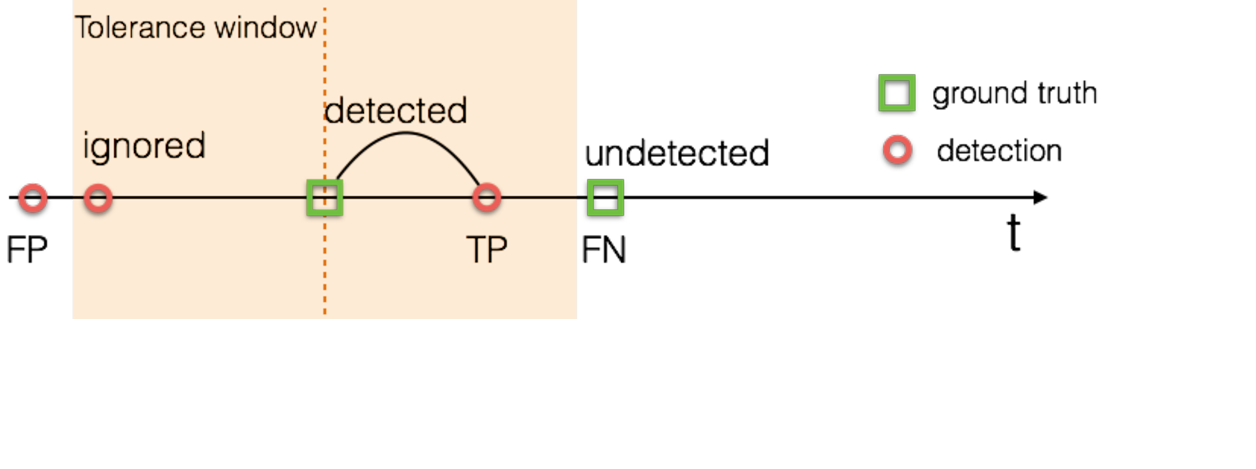
\includegraphics[width=.95\textwidth]{gfx/chap4/matching_dilemma.pdf}
\caption{A matching dilemma between detected moments of change and two ground truth changepoints.}
\label{fig:matching_dilemma}
\end{figure}

One cure to the above approach is to pick only the $\tau$ that minimizes the temporal distance to each $T$, if multiple are within the tolerance range.
The remaining shall be regarded as false positives for not being the most relevant to any ground truth changepoints.
Another issue occurs when the tolerance range of two ground truth changepoints overlaps.
And a $\tau$ falls in the tolerance range of both ground truth timestamps.
Which one should this $\tau$ detect?
A such dilemma is illustrated in Figure~\ref{fig:matching_dilemma}.
The tolerance range of the first ground truth moment is indicated in light orange in the graph.
Two detected moments of change fall in this range.
The later one is regarded as a $TP$ for being the closest match to the first ground truth moment.
Meanwhile, this changepoint from detection is as well in the tolerance range of the second ground truth changepoint.
However, it can no longer be used to detect the later ground truth event, thus leaving the later undetected.
It is not necessary an optimal arrangement of matching between ground truth and detection events.
Because both ground truth has at least one detected moment of change within their window, yet one of them is left undetected.

The realization of the above dilemma made us question what is an optimal matching from an overall view.
An reasonable formulation could be one that first maximizes the number of $TP$, i.e. matching (one-to-one) between ground truth and detection timestamps as long as the tolerance window allows.
Then the it minimizes the total/average distance between these matched pair of timestamps to maximize the relevance of the matching.
More formally, an optimal mapping between $T_{i:k}$ and $\tau_{i:m}$ with shift tolerance $w$ is defined as $MP = \{(T_x, \tau_y)\} \mid |T_x - \tau_y| \leq w \}$, as the one that first maximizes $|MP|$, the size of $MP$, and then minimizes $\sum_{(T_x, \tau_y) \in MP} |T_x - \tau_y|$. 

%False Negative ($FN$) composes of $\{T_i \mid \nexists \tau_j \in \tau_{1:m}, \tau_j = T_i \}$.
%However, there are many times during labeling that finding a clear cut position for certain RTT changes is difficult for human beings, and the labeled moment of change might reasonably vary within a range.
%It is therefore too harsh to require exact match from change detection.

%Introducing a window of tolerance $w$, we are confronted with an issue where 
%$T_i$ can be detected by multiple detection outputs $ \{\tau_j \mid |\tau_j - T_i| \leq w \}$. 
%Symmetrically, $\tau_j$ can be associated with several $T_i$ within the tolerance window.
%If many-to-many mapping between $T_{1:k}$ and $\tau_{1:m}$ is allowed, the number of $TP$ could be overestimated. while $FN$ underestimated.

%One straightforward solution adopted by Numenta is that a $T_i$ can only be detected
%by the closest detection in the window $\hat \tau_i$~\cite{Lavin2016}. All the rest detected changes will be ignored.
%The problem with this approach is that the actual change that is closest to the above $\hat \tau_i$, denoted as $\hat T_i$, doesn't necessary satisfy $\hat T_i = T_i$. 
%Such discrepancy indicates that the mapping between ground fact and detection is potentially not optimal in two aspects:
%\begin{enumerate}
%\item $\hat T_i$ could end up undetected even though there are detection points %within the window;
%\item the overall time shift between truth and detection is not necessary the minimum.
%\end{enumerate}

\begin{figure}[!htb]
\centering
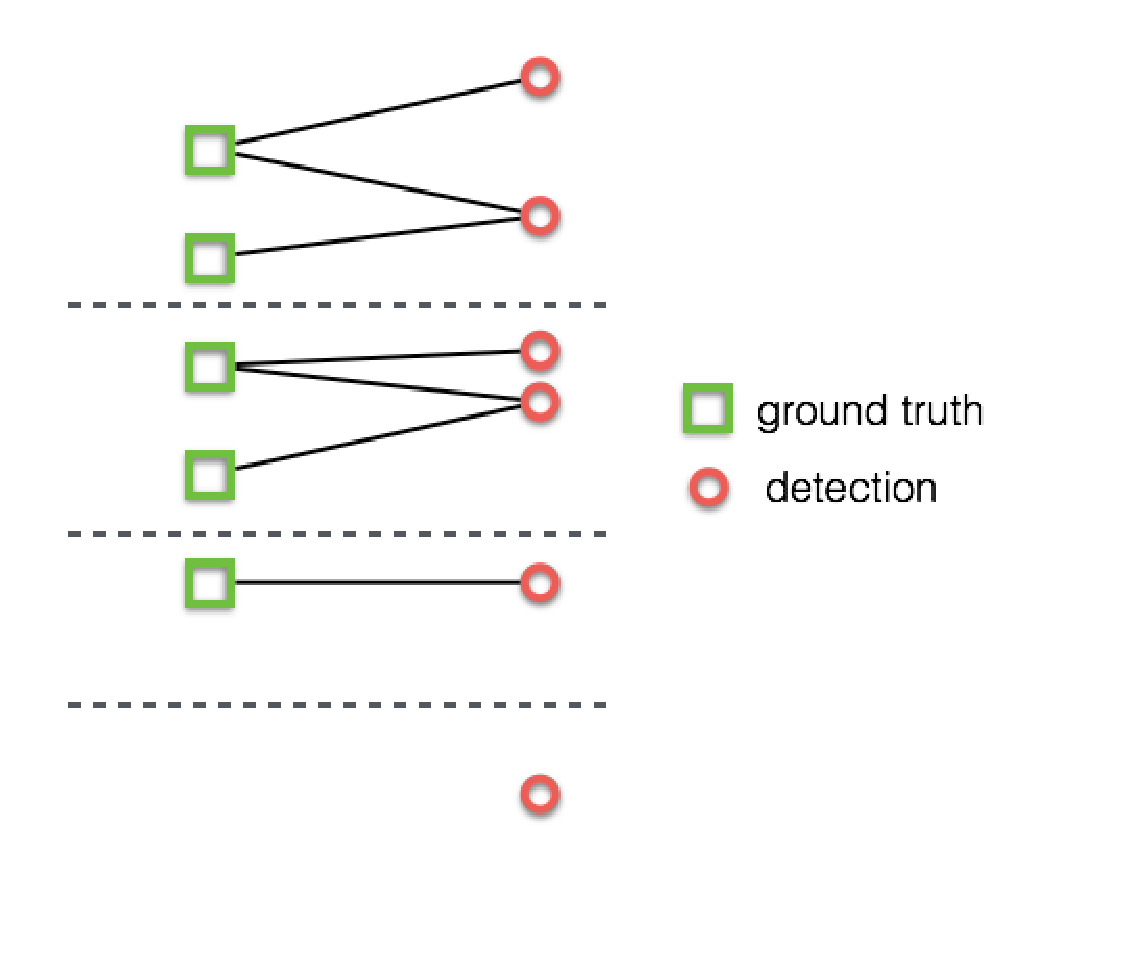
\includegraphics[width=.7\textwidth]{gfx/chap4/bipartit_graph_cons.pdf}
\caption{Constructing a bipartit graph from ground truth and detected changepoints. When the distance between a ground truth and detected changepoint is equal to or smaller than the defined tolerance window size, there is an edge connecting them. The weight of this edge equals to the distance in time between the two nodes.}
\label{fig:bipartit_graph_cons}
\end{figure}

A convenient way to find the $MP$ is through the construction of a bipartite graph $G = (V \cup W, E)$, illustrated in Figure~\ref{fig:bipartit_graph_cons}.
$V \cup W$ are the vertices of the graph.
They are made of the ground truth and detected changepoints, i.e $V = T_{i:k}$ and $W = \tau_{1:m}$.
Edge $E$ is composed of all ground truth and detected change moments pairs the distance between which are no larger than the tolerance window, i.e. $E = \{(p, q) \mid |p - q| \leq w, p \in V, q \in W \}$.
The cost of each edge is defined as the distance/shift in time between its two extremities $C(e) = |p-q|, e \in E$.
Once the graph is constructed, the problem of finding the optimal mapping $MP$ is translated into a well studied task of finding the \textit{minimum cost maximum-cardinality matching} of $G$.

The Hungarian matching algorithm, as well known as the Kuhn-Munkres algorithm, is an established way of solving \textit{minimum cost maximum-cardinality matching} problem~\footnote{An explanation to how the algorithm works would be lengthy and deviate the discussion to a direction that is less original. Interested reader can find a well written and illustrated guide to it via this link: \url{https://brilliant.org/wiki/hungarian-matching/}.}. 
The complexity of the algorithm is cubic to the number of the vertices in the graph.
When there are a large number (e.g. $> 100$) of potential changes to be detected, it can thus take a while to compute.
A performance boost is though possible due to the presence of the tolerance window.
An edge is not going to connect two vertices, each from one part of the graph, that are far away in time.
This feature allows us to cut the graph into much smaller disconnected sub-graphs.
The cutting is illustrated in Figure~\ref{fig:bipartit_graph_cons} by the dotted lines.
For positive numbers, the sum of cubic is always smaller than the cubic of number sum.
Applying the Hungarian algorithm on disconnected sub-graphs can therefore reduce the amount of calculation.

Once the $MP$ is identified for $G$, the definitions for $TP$, precision and recall all come up naturally.
For each detection $\tau_j$, if $\exists m \in MP, \tau_j \in m$, it is regarded as a $TP$, otherwise as a $FP$ (false positive).
All the ground truth without matched detection $\{T_i \mid \nexists m \in MP, T_j \in m\}$ contributes to $FN$ (false negative).
Precision of the changepoint detection method, defined as  $\frac{TP}{TP+FP}$, can be interpreted as the fraction of detection that is relevant or useful.
Recall, defined as $\frac{TP}{TP+FN}$, can be regarded as the fraction of all ground truth change points that the method can successfully detect.


\subsubsection{Ground truth changepoints with weights}
\begin{figure}[!htb]
\centering
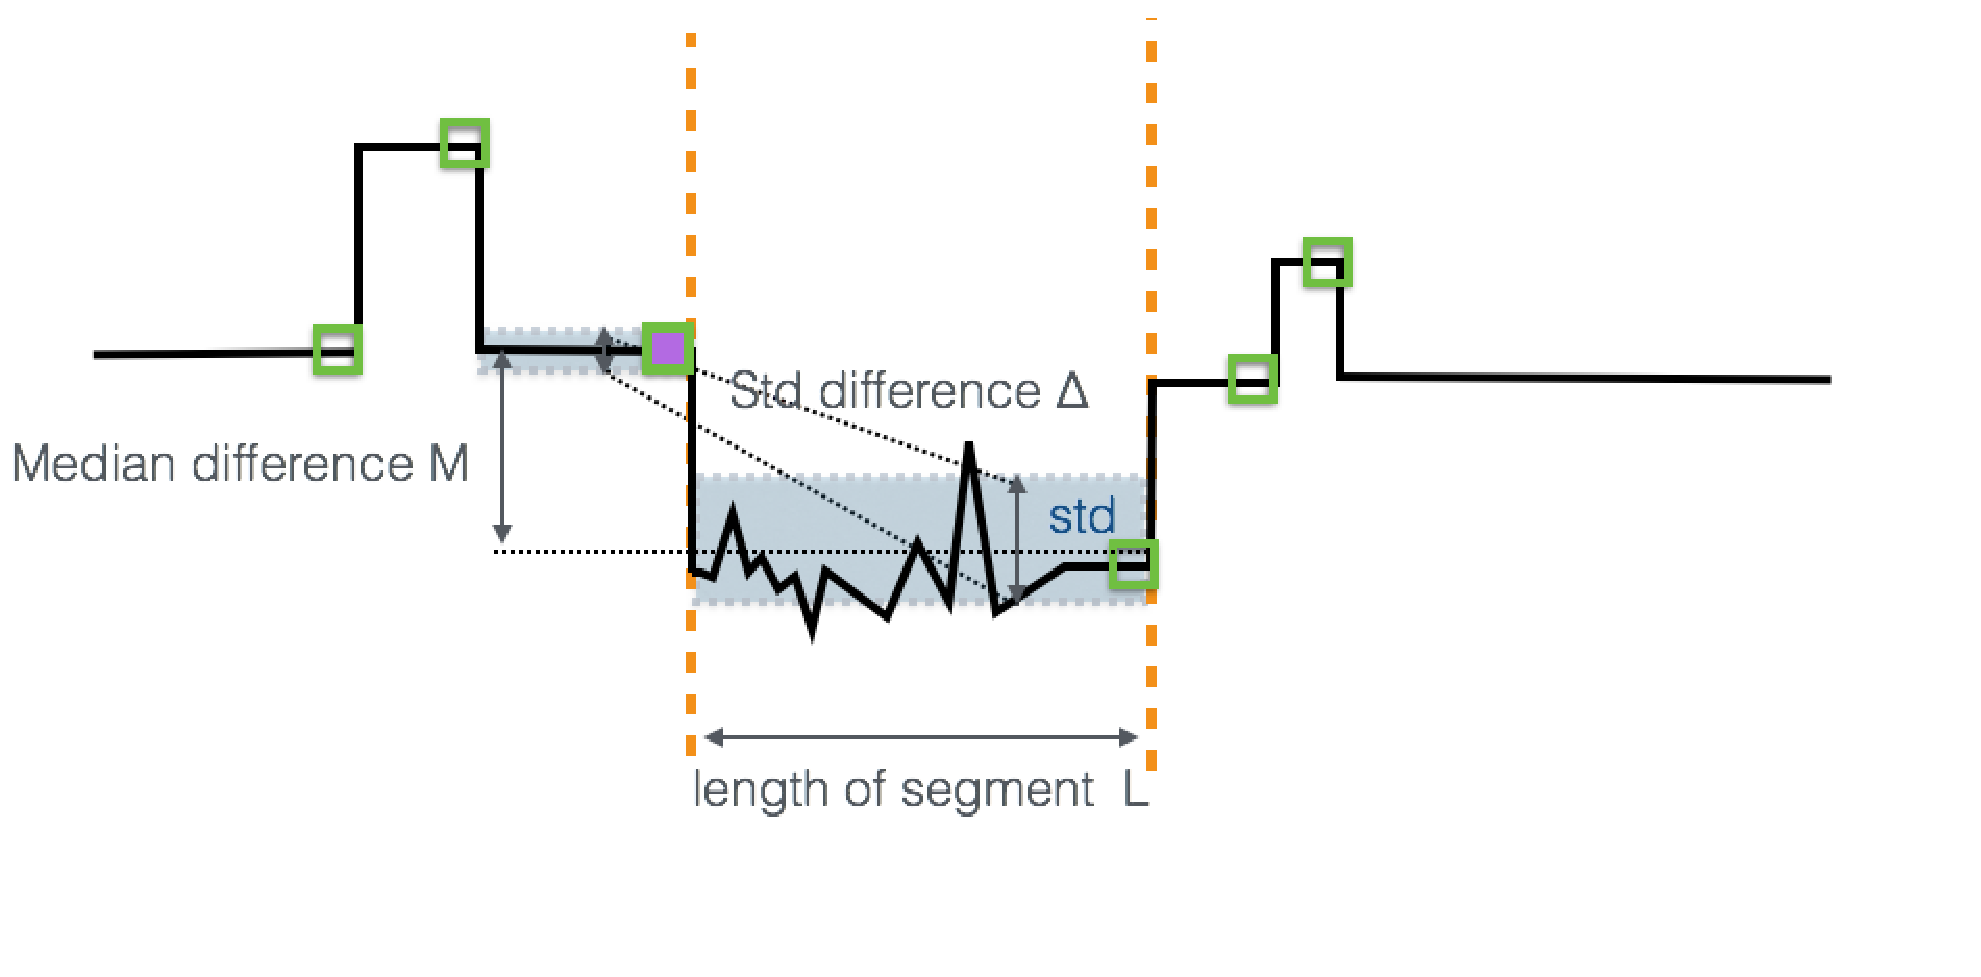
\includegraphics[width=.8\textwidth]{gfx/chap4/groundtruth_weight.pdf}
\caption{An illustration of how each ground truth (green square) moment of change is weighted. The example focuses on the while with a purple filling.}
\label{fig:groundtruth_weight}
\end{figure}

Each detected change may be treated equally (e.g. followed by root cause analysis, route re-selection), yet not all ground truth RTT changes are equally important in practice.
Some changes could be for example relatively short living or small in amplitude.
We thus propose to weight each ground truth changepoint $T_i$ according to the follow three elements illustrated in Figure~\ref{fig:groundtruth_weight} for the purple filled ground truth changepoint:
\begin{enumerate}
\item the length of RTT segment following $T_i$, i.e. $T_{i+1} - T_i$;
\item the RTT level difference across $T_i$, denoted as $M_i$; 
\item the RTT volatility difference across $T_i$, denoted as $\Delta_i$.
\end{enumerate}
More formally for each $T_i \in T_{i:k}$, with $T_0=1, T_{k+1} = n$, we define:
\begin{equation*}
M_i = |Median(y_{T_{i-1}+1:T_i}) - Median(y_{T_i+1:T_{i+1}})|.
\end{equation*}
We use median instead of mean in the purpose of reducing the impact of abnormally large RTT measurements.
We define:
\begin{equation*}
\Delta_i = |Std(y_{T_{i-1}+1:T_i}) - Std(y_{T_i+1:T_{i+1}})|,
\end{equation*}
as the measure for variance change across the changepoint.
We define empirically the weight associated to each $T_i \in T_{1:k}$ as:
\begin{equation*}
\Omega_i = MAX(\log_2\frac{T_{i+1} - T_i}{\rho}, 0) \times (M_i + \Delta_i).
\end{equation*}
Here $\rho$ is a threshold for RTT segment length. 
If $T_i$ leading to an RTT segment shorter than $\rho$, we ignore it in calculating $Recall$.
The intuition behind this weighting is that RTT changes of large level or volatility are in practice regarded as more important. 
$\rho$ and $w$ tolerance window are set to $8min$ in this work, corresponding to two ping measurement intervals. 

We can henceforth formulate a `weighted' version of the $Recall$ metric to better reflect the operational importance of detected RTT changes: $Recall_W = \frac{\sum_{i, T_i \in TP} \Omega_i}{\sum_{j=1}^k \Omega_j}.$

Precision and recall are both important in evaluating the performance of a detection method.
To consolidate them into one single metric, we used the notion of $F_2$ score.
It weights recall twice as important as precision: $F_2 = (1+2^2) \times \frac{Precision \times Recall}{2^2Precsion + Recall}.$
The practical implication of this choice is that handling some $FP$s is less unwanted than missing out some important RTT changes.

\subsection{Ground truth dataset}
\label{sec:label}

\subsubsection{Dataset quality control}

\begin{figure}[!htb]
\centering
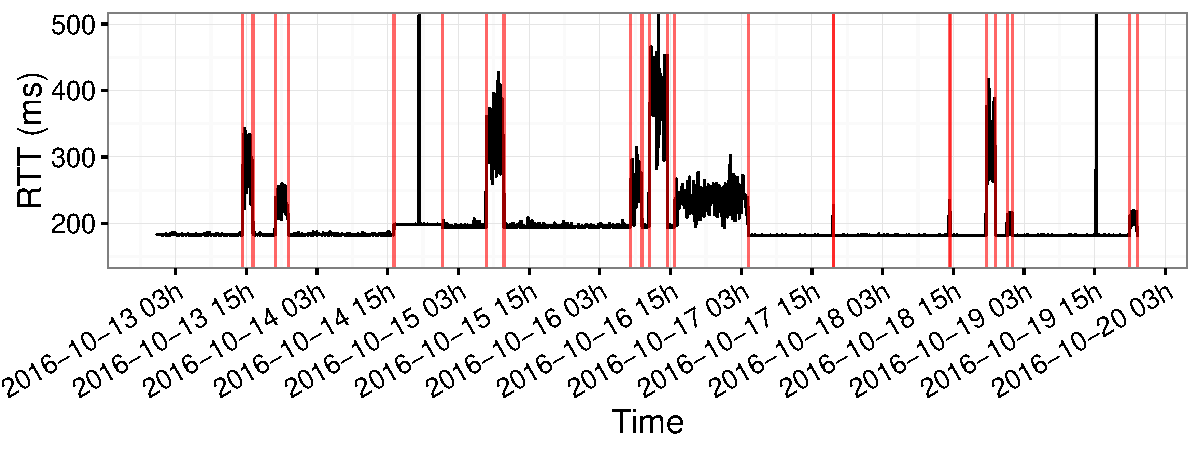
\includegraphics[width=.96\textwidth]{gfx/chap4/artificial_trace.pdf}
\caption{First 2500 %(out of 6506) 
Datapoints of an artificial RTT time series (one datapoint every 4min). 
Red vertical lines correspond to generated changes.}
\label{fig:art_example}
\end{figure}

In order to determine which detection method works the best over RTT timeseries, 
a dataset with \textit{a priori} labeled moments of RTT change is required, serving as ground truth.
It's quality is essential to the credibility of evaluation results.

There are two approaches to fabricate a labeled ground truth dataset: 1) artificially generated data; 2) real data with labels manually put on.
Obviously, real data is more representative of the Internet delay character.
It is thus the preferred choice.
However, it can only be labeled by humans with domain knowledge.
Manual labeling is tedious and error-prone.
Without due care, it can undermine the quality of the entire ground truth dataset.
%Moreover, identifying significant change in RTT time series lacks an operational standard.

Therefore, it is important to verify the labeling quality.
To that end, we rely on an artificial dataset.
The idea is to generate some synthetic RTT timeseries with known changepoints.
These artificial timeseries are then mixed up with real RTT timeseries during human labeling.
Once the labeling is done, we compare the human-labeled changepoints over the artificial dataset with its the generated changepoints, using the scoring method presented in Section~\ref{sec:score}.
That is to evaluate the detection performance of human labellers using generated changes as ground truth.

Synthetic RTT timeseries are after all not real RTT measurements.
Human labellers performing perfectly over generated traces doesn't necessary indicate that they would do as well on real RTT measurements.
Therefore it is highly desired that the artificial RTT timeseries resemble real ones as much as possible.
Following steps are taken to generate a synthetic RTT time series.

First, we randomly generate several phases/segments of different delay baselines.
Different RTT baselines corresponds to the different physical lengths on different Internet paths.
For each phase of RTT baseline, we add noises representing micro queue length changes, waiting time due to router load and scheduling policies etc.
Finally for each phase of RTT baseline, we generate relatively long during congestion with its own Markov process.
Random parameters appropriate to each baseline segment decide the chance of getting into and out of a congestion period.
The generated changepoints are moments when there are baseline delay changes and congestion entrance/exit.
Short living spikes (length $\leq 2$ datapoints) are considered noises rather than real changes.
For the detailed generative models and model parameters of each step, please refer to the documentation in the code space available at \url{https://github.com/WenqinSHAO/rtt_gen.git}.

20 synthetic RTT timeseries, with 6485 datapoints each on average, are generated with the fabricated tool.
The time interval between datapoints is 4min, in line with RIPE Atlas built-in ping measurement.
They represent 8646 hours of RTT measurements with 935 generated changepoints.
An example of these synthetic RTT trace is shown in Figure~\ref{fig:art_example}.
The red vertical lines, indicating generated changepoints, are moments when there is a base line RTT change, or a congestion period starts/ends.

\subsubsection{Labeling}
%Ensured that human labellers are capable of detecting changes, we proceed with real RTT traces.
As for the real RTT measurements, a great amount of real RTT traces of various characters are selected from RIPE Atlas to construct the ground truth dataset.
Some are full of fluctuations; some contain periodic congestion, some have many step-wise changes, etc.
50 real RTT timeseries containing 408,087 datapoints are selected.
They represent more than 34,008 hours, i.e. 1417 days, of RTT measurements. 

How the labeling is done by humans over a large data set as is crucial to the data quality.
Looking at all these timeseries and marking changepoint timestamps with a text editor is clearly not a good idea.
To enable intuitive (what humans are good at) labeling, we fabricated an interactive tool to visualize RTT time series \url{https://github.com/WenqinSHAO/rtt_visual.git}.
With this tool, the labellers can easily pan, zoom RTT time series and verify the positions of marked changepoints~\footnote{The labellers are researchers/graduate students in networking.}.

1047 changepoints were identified by the labellers for these real RTT timeseries.
All the labelled RTT traces, synthetic and real, along with the generated changepoints are all available in the main project repository specified in Section~\ref{sec:cpt_data}.
Only the human-labeled real RTT time series are regarded as ground truth dataset.
During the labeling process, the labellers all found that they were not sure whether a given RTT timeseries is real or synthetic.
We therefore judge that the synthetic dataset are good enough.
After revealing the identity of each time series, the labellers concluded that the synthetic RTT timeseries seemed to have less rich variation patterns compared to the real ones.
There are moments when the labellers were not quite sure if a changepoint were to be placed or not, or where exactly to place a changepoint.
These suspicious moments all turned out to be within real RTT timeseries.
The presence of such difficulty is exactly one reason that time shift tolerance is needed in detection performance evaluation.

\subsubsection{Performance of human change detector}
\begin{figure}[!htb]
\centering
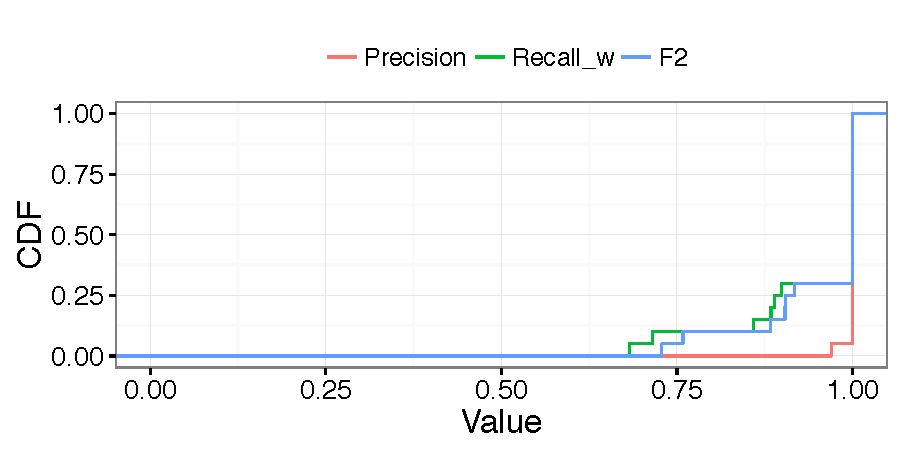
\includegraphics[width=.72\textwidth]{gfx/chap4/antoine_eval.pdf}
\caption{$Presicion$, $Recall_W$ and weighted $F_2$ of human labellers on synthetic dataset.}
\label{fig:antoine_eval}
\end{figure}

The detection performance of human labellers on the synthetic dataset is shown in Figure~\ref{fig:antoine_eval}. 
Human labellers have $100\%$ for both $Precision$ and $Recall$ on 14 traces.
For the rest, the $Precision$ remains high. A few changes are miss out, but their total weight remain limited.
This suggests that the human labellers, with diligence and the help of the visualization tool, are indeed capable
of high quality labeling.

\section{Evaluating changepoint methods}
\subsection{Candidate changepoint methods}
\label{sec:method}
With the evaluation framework ready, it opens the door to the exploration of best performing changepoint detection method for RTT measurements.
For the detection family presented in Section~\ref{sec:cpt}, there are two major parameters to be set: penalty and cost function/distribution.
We discuss in detail these parameters in this section, while leaving the examination of other methods for future work.

We consider the combination between all the information criterion introduced (AIC, BIC, MBIC and Hannan-Quinn), and all the supported distribution types, including the non-parametric approach based on empirical distribution.

With some preliminary tests, we quickly realized that detection with Normal distribution tend to be over-sensitive, under all the penalty settings.
Many short living and insignificant noises are marked as changepoints.
It is because the mean and variance of Normal distribution are independently controlled by two separate parameters, which increases the chance of fitting subtle changes either in level or volatility.
On the other hand, Exponential, Gamma and Poisson distribution are too numb.
The mean and variance of Poisson and Exponential distribution are coupled by one parameter,
which restrains their freedom of adjustment~\footnote{Poisson, mean=variance=$\lambda$; Exponential, mean/variance=$\lambda$, mean=$1/\lambda$.}.
Gamma distribution faces the same issue, but with a more complicated story.
A Gamma distribution can be describe by two parameters $\alpha$ and $\beta$: mean=$\frac{\alpha}{\beta}$, variance=$\frac{mean}{\beta}$.
\cite{Killick2013a}, the implementation we use, requires an \textit{a priori} input for $\alpha$, which actually decides the overall sensitivity. 
Only $\beta$ is adjusted in detecting changepoints.
With a larger $\alpha$, a larger $\beta$ is needed to maintain the same mean estimation for given a segment.
Fixed mean with larger $\beta$ imposes a smaller variation tolerance, thus more likely to split the given segment due to smaller variance changes.
In short, larger $\alpha$ leads to more sensitive detection.
The default option sets $\alpha$ set to 1, which degenerates Gamma distribution to Exponential distribution. 
We further tried $\alpha$ from 1 to 100, at unit step. 
None of them outperforms the best settings shown later on. 
We therefore no longer consider Gamma distributions.

When assuming Exponential and Poisson distribution, we notice that the average level of an RTT time series somehow dictate the variation tolerance.
For instance, for a path including trans-Pacific links, we shall expect a minimum RTT above $80msec$.
In this case the corresponding Poisson distribution could easily tolerate several RTT deviations of $20msec$, which is already non-negligible.
However, having coupled mean and variance can as well be a desired feature. 
We observed during labeling that the level of an RTT segment and its variance are often positively related during congestion periods. 

To leverage the above described feature and as well as boost the detection senstivity, we propose for Exponential and Poisson distribution a \textit{data transformation}: subtracting the RTT time series by its minimum value (baseline) to lower down its overall RTT level~\footnote{Note that timeout measurements are set to 1000ms. 
For Poisson distributions, RTT values are rounded to the closest integer.}. 
Changes are then detected for the baseline-removed RTT time series when assuming Poisson and Exponential distribution.
Such setting is denoted as \texttt{cpt\_poisson} and \texttt{cpt\_exp} respectively.
For the sake of comparison, we also consider Poisson distribution \textbf{without data transformation} and denote it as \texttt{cpt\_poisson\_naive}.
Normal distribution and non-parametric approach are applied directly on initial RTT measurements.
%\footnote{The data transformation is useless for these two methods.}.
%results uniform level shift over all potential segments in parameter estimation for Normal and non-parametric approach, thus pointless.}.
%% No need to explain why? OK
%%% Well, since I don't understand the explanation, better not... ;-))))))
They are denoted as \texttt{cpt\_normal} and \texttt{cpt\_np} accordingly.

\subsection{Evaluation of candidate methods}
\label{sec:eval}

Before evaluating the methods presented above, one might wonder 1) whether the RTT segments in the ground truth dataset follow principally a specific distribution, and 2) whether that distribution assumption leads to the best detection performance.

We performed distribution test for 813 RTT segments longer than 20 datapoints against each of the discussed distribution types. 
We require a significance level of 0.05 in distribution test. 
Shapiro-Wilk test is used for Normality test;
Chi-squared test for Poisson; 
Kolmogorov-Smirnov test for Exponential. 
Distribution parameters are estimated through Maximum Likelihood Estimation.
71 follow Normal distribution, 13 follow Poisson distribution, 11 follow Exponential distribution~\footnote{It is possible that a segments passes the test for multiple distributions. Thus there are overlaps in the numbers.}. 
None of these distributions seems to have a dominant popularity among the labeled RTT segments.
Still, Normal distribution seems to be the most compatible.

All combinations between distribution types and penalty choices are employed to detect changepoints ins the ground truth dataset.
For each distribution type, we only plot its best performing penalty setting in terms of weighted $F_2$ score in Figure~\ref{fig:real_eval}.
In later discussion, when we mention a specific distribution type say \texttt{cpt\_poisson}, we actually refer to a configuration including the distribution itself, the corresponding data transformation plus its best performing penalty choice.

More than $75\%$ of changes, in terms of weight, can be detected for more than half of the timeseries with any of these distributions.
All these distribution types have better weighted $F_2$ than classic $F_2$, indicating some changepoints missed out are indeed of little operational importance.
However, it seems to have a big space for improvements.
Efforts are especially needed to raise the precision of the detection results.

The precision of \texttt{cpt\_normal} is particularly poor.
This confirms that \texttt{cpt\_normal} is indeed over-sensitive for RTT type of data~\footnote{Note that \texttt{cpt\_normal}'s best penalty is MBIC, the largest adaptive penalty setting. This means that the detection sensitive is already suppressed to its maximum.}.
On the contrary, the recall of \texttt{cpt\_normal} is outstanding among all the candidates.
However, its $F_2$ scores are the poorest~\footnote{With $F_2$, recall is already weighted twice as important as precision.}.
The poor overall detection performance highlights the importance of striking a proper balance between sensitivity and relevance.
It suggests as well that the goodness of fit is not necessary a guarantee for detection performance.
For rest methods, their performances are relatively close. 
Compared to \texttt{cpt\_poisson\_naive} (without data transformation), \texttt{cpt\_poisson} achieves higher recall and weighted recall without obviously sacrificing precision.
Consequently, \texttt{cpt\_poisson} stands a slight advantage in overall performance.
As a matter of fact, without data transformation, assuming Exponential distribution detects no changepoint for a big part timeseries in the ground truth dataset.
These are all evidences that the proposed data transformation improves the detection performance for Poisson and Exponential distribution.

\begin{landscape}
\begin{figure}[!ht]
\centering
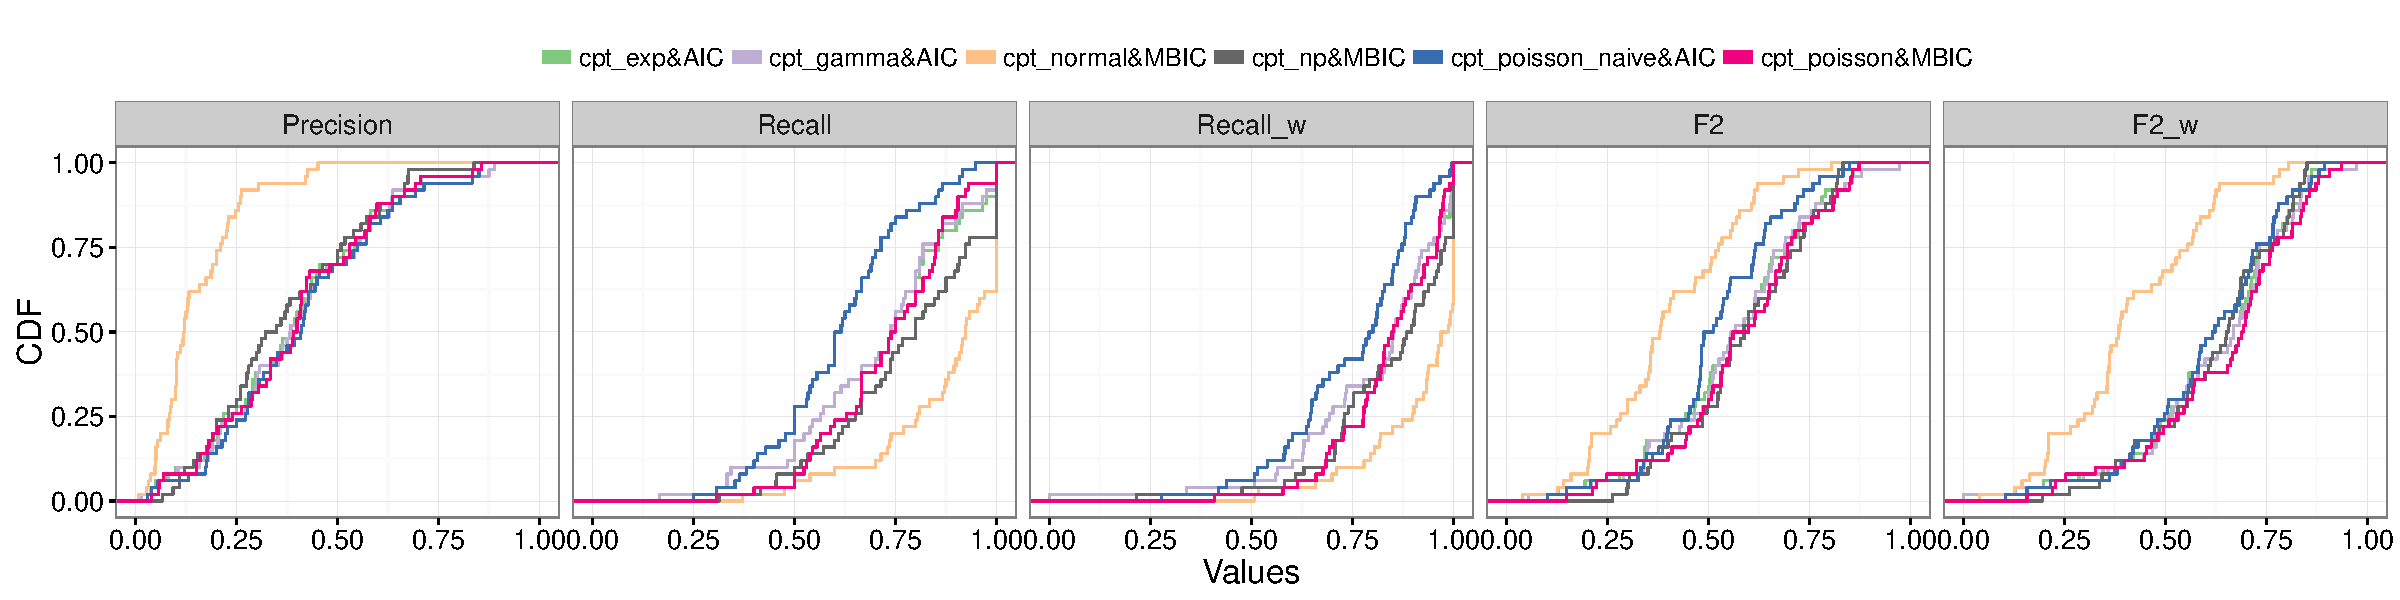
\includegraphics[width=1.8\textwidth]{gfx/chap4/real_eval_bis.pdf}
\caption{$Precision$, $Recall$, $Recall_W$, $F_2$ and $F_2W$ with weighted recall on real RTT traces.}
\label{fig:real_eval}
\end{figure}
\end{landscape}

\section{Characters of RTT changes}
\label{sec:cpt_trace}
\texttt{cpt\_poisson} and \texttt{cpt\_np} with MBIC are used to detected RTT changes for all the 6029 collected ping timeseries spanning over three months.
Please refer to Section~\ref{sec:cpt_data} for more details concerning the collected data.
We consider \texttt{cpt\_poisson} as it is the best performing one, though by a small margin.
\texttt{cpt\_np} is included as it performs well and its cost function follows a different construction principal.
%%% Well... It has also good performance right. Other wise you would not consider it...
%%% Yes, but rather close with the rest. Actually except normal, all the rest are rather close... so the reason choosing it instead of exponential is because the construction of cost function is fundamentally different.

%Since there is no guarantee that the traces included in labelled dataset covers all possible RTT morphology, it is thus possible that methods performs less well on evaluation dataset detects changepoints more appropriately on a larger dataset with richer characters.

\begin{figure}[!htb]
    \centering
    \begin{subfigure}[b]{.48\textwidth}
	\centering
	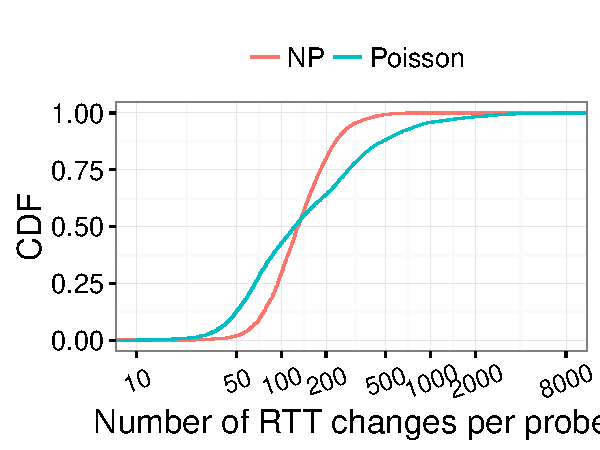
\includegraphics[width=\textwidth]{gfx/chap4/rtt_ch_count_cdf_cmp.pdf}
	\caption{\footnotesize CDF.}
	\label{fig:rtt_ch_count_cdf_cmp}
	\end{subfigure}
	\begin{subfigure}[b]{.48\textwidth}
	\centering
	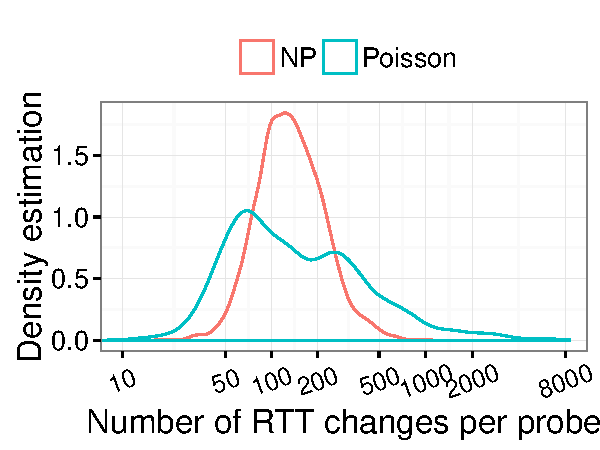
\includegraphics[width=\textwidth]{gfx/chap4/rtt_ch_count_density_cmp.pdf}
	\caption{\footnotesize Density.}
	\label{fig:rtt_ch_count_density_cmp}
	\end{subfigure}
\caption{RTT changepoints number distribution with different detection methods under MBIC.}
\label{fig:rtt_ch_count_cmp}
\end{figure}

Figure~\ref{fig:rtt_ch_count_cmp} shows the distribution of RTT change numbers per probe trace. 
4,844 probe traces each containing more than 30,000 ping measurements are considered in the figure.
854,626 RTT changepoints are detected by \texttt{cpt\_np}.
\texttt{cpt\_poisson} almost doubled this number with 1,638,858 RTT changes.
Interestingly, the median change numbers for both methods is the same, 122.
Figure~\ref{fig:rtt_ch_count_density_cmp} shows that the change number by \texttt{cpt\_poisson} spreads over a much wider range.
With \texttt{cpt\_poisson}, 711 probes traces ($11.86\%$) have more than 500 changepoints, while only 35 ($0.58\%$) with \texttt{cpt\_np} experienced that many changes.
This is probably because the cost function of \texttt{cpt\_np} bases on the estimation of quantiles (by default 10 quantiles used, more can be set) of empirical distribution. The dimension of $\theta$ is much larger than Poisson and Normal distribution. The penalty value increases hence much faster for \texttt{cpt\_np} when new changepoint is added, which prevents extremely large number of changepoints per probe trace.

\begin{figure}[!thb]
\centering
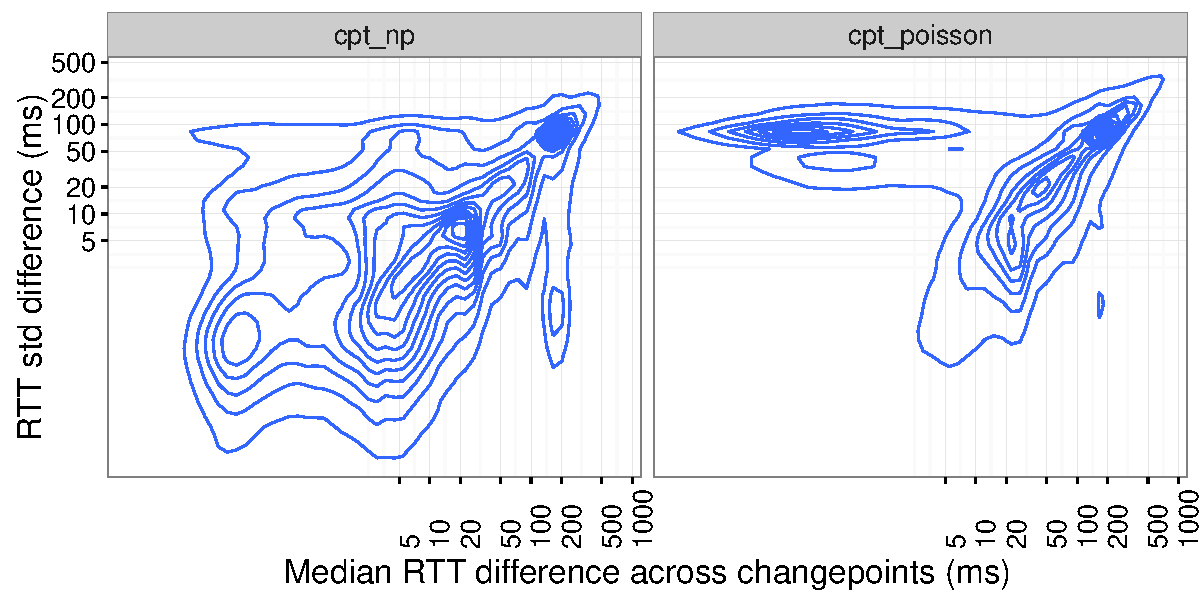
\includegraphics[width=.96\textwidth]{gfx/chap4/rtt_ch_chara_cmp.pdf}
\caption{Density estimation of RTT changepoints characteristics.}
\label{fig:rtt_chara_cmp}
\end{figure}
We describe a detected changepoint from two aspects: 1) the difference of median RTT across the changepoint, and 2) the difference of RTT variance level across the changepoint.
More specifically, they are $M$ and $\Delta$ defined from ground truth changepoint weighting in Section~\ref{sec:score}.
Figure~\ref{fig:rtt_chara_cmp} visualizes the two features of RTT changepoints detected by the two methods.
Since there is a huge amount of changepoints that overlaps each other on the $M$ and $\Delta$ surface,
it becomes impossible to interpret if we were to explicitly plot each one of them.
Therefore, we summarize all the changepoints using a 2-dimensional density estimation (with MASS:kde2d package in R).
A same practice has been conducted in Section~\ref{sec:miss_atlas} for Figure~\ref{fig:all}.
A contour line represents a trajectory on which the changepoint density is the same on the $M$ and $\Delta$ surface.
Inside a contour, the density becomes higher.

On the $M$ and $\Delta$ surface, changepoints in the top right corner are important ones with serious networking implications.
Both methods result a pretty high changepoint concentration in this area.
This suggests that there were indeed significant performance changes on the measured path over the three-month time.
\texttt{cpt\_poisson} and \texttt{cpt\_np} both succeed in identifying some of these changes.
What seems to be weird is that there is a cluster of changepoints detected by \texttt{cpt\_poisson} on the top left panel of the the $M$ and $\Delta$ surface.
These changepoints, more precisely 319,541 in number ($19.49\%$) with $M<5msec, \Delta>50msec$, imply big variance yet small level changes.
They are almost absent in the detection results of \texttt{cpt\_np}.
After investigation over these chagnepoints, we discovered that they are mostly caused by frequent timeouts, and are associated with short RTT segment length. For example, probe 20854 had 2308 timeout measurements dispersed in the entire trace.
Meanwhile, \texttt{cpt\_np} handled these timeouts gracefully without emitting all the time change alarms.
\texttt{cpt\_poisson} appears to be a bit troubled by these short and frequent deviations.

Changepoints in the down left corner are relatively subtler.
They in general won't lead to significant network performance issues and can thus be safely ignored in TE practices.
Reasonably, a small fraction of changepoints detected by \texttt{cpt\_poisson}, 87,021 ($5.31\%$), are with $M$ and $\Delta$ both smaller than $5msec$.
Correspondingly, most part of this area in the figure is already outside the most outer contour.
This suggests \texttt{cpt\_poisson} tolerates well these small changes.
One the other hand, \texttt{cpt\_np} appears to be quite reactive in such case.
As a matter of fact, 331,062 ($38.71\%$) such changes are detected by \texttt{cpt\_np}.

We later on cross the detected RTT changes with path changes.
With that, we further discuss the detection sensitive and relevance of these two methods with regard to network events.

\section{Detecting path changes}
\label{sec:path}

In this section, we detect path changes experienced by the collected RTT measurements.
Both AS and IP level path changes are attended.
They are known to have potential impact on RTT.
RIPE Atlas built-in path measurement uses a rotating Paris ID setting.
This brings confusion between IP path changes caused by load balancing and those due to intradomain routing changes.
We address this issue in this section.
%in order to explore in depth the detection sensitivity difference with different parameters and the detection relevance compared to path changes, network events known to have consequence on RTT.
The purpose of path change detection is not to repeat some of the studies sumeraized in~\ref{sec:rtt_path}, 
such as which kind of path change contributes most to RTT change.
It rather helps to enhance the understanding on changepoint detection for RTT measurements.


\subsection{Routing change and \acf{LB}}

Schwartz et al.~\cite{Schwartz2010} regarded all paths between a source-destination pair as ``parallel paths'' and found out that RTT measurements over these paths were mostly overlapping.
However, there are two kinds of transitions among ``parallel paths'' that need to be distinguished.
They are 1) IP path changes caused by intradomian routing protocol dynamics, such as route recalculation after link failure or configuration update, 
and 2) those caused by LB mechanisms. 
Intradomain path changes before the era of LB haven been shown to be responsible for important RTT changes~\cite{Pucha2007}. 
On the other hand, LB paths are of equal/close administrative cost, hence similar performance characteristics~\cite{Augustin2011}.
This suggests that these two kinds of IP route changes could have very different impact on RTT, and thus need to be distinguished.
 
Trivial as it may sound, detecting IP path changes is challenging for RIPE Atlas built-in traceroute measurements.
The difficulties come from two aspects: 1) the wide deployment of IP-level LB; 2) RIPE Atlas uses Paris traceroute with different Paris IDs every other measurement (incremented by 1, recycling between 0 and 15)~\cite{Augustin2006, Pelsser2013}.
IP paths taken by two neighboring measurements can thus naturally differ -- 
load-balanced on different available paths with different Paris IDs.  
From this angle, plain IP path changes doesn't mean that there were topological or configuration changes that lead to any real routing change. 
On the other hand, having different Paris IDs every time can also be helpful in this context.  If traceroute were locked on a single Paris ID, it would then be unlikely to detect routing changes that only affect paths corresponding to other Paris IDs.

\subsection{Intradomain Routing Pattern change}
When a different IP path is measured with a same Paris ID,
there is potentially a routing change. 
We call this kind of IP path change an \acf{IRP} change.
In the example below, the IRP change happens when Paris ID 2 begins to take IP path E instead of B. We refer to the two measurements with same Paris ID but different IP paths as \textit{conflicting} measurements.
\begin{Verbatim}[fontsize=\small]
                             | IRP change
Paris ID: 0 1 2 3 4 .. 15 0 1|2 3 ..
IP Path:  A B B A A .. C  A B|E E ..
       A measurement series  | boundary -> forward
\end{Verbatim}

IRP changes can thus be identified by constructing a series of measurement sequences.
Each sequence shall not contain conflicting measurements. 
Yet, combing any two neighboring sequences, there shall be as least one pair of conflicting measurements, as otherwise they can be merged.
This can be done by moving the boundary of measurement sequences \textit{forward} to include non-conflicting measurements, till a conflict is encountered, as shown in the above example.
We call this approach \textit{forward inclusion}.

The drawback of \textit{forward inclusion} is that it potentially delays the detection of actual IRP changes.
This is because, when including non-conflicting measurements forwardly, a measurement sequence always has the chance to absorb measurements till it experiences all the possible Paris IDs.
However an actual IRP change could happen before that moment.
An example of possibly delayed IRP change is given right below:
\begin{Verbatim}[fontsize=\small]
        !Possible position of actual IRP change        
.. 1|2 3!4 5 .. 15 0 1|2 3 4 5 ... 15 0 1 2 3 4 5 ..
.. B|B A!A C .. C  A B|E E A C ... C  A B E E A C ..
                      | IRP change forward inclusion
                      | backward <- boundary
\end{Verbatim}
With \textit{forward inclusion}, an IRP change will be detected at the 2nd appearance of Paris ID 2.
While the actual change probably happens at the 1st appearance of Paris ID 4.
It is because starting from the first Paris ID 4, all the measurements are non-conflicting with the later measurement series.
The 1st appearance of Paris ID 2 and 3 are in fact a short deviation from a popular IRP.

Cases like this are highly possible, because networks tend to have some stable configurations that lead to a few dominant paths over time~\cite{Chandrasekaran, Pucha2007}. 
Deviations from dominant/popular IRPs are thus likely to be short living.
With RIPE Altas built-in measurements, they probably won't last long enough to experience all the Paris IDs~\footnote{It takes at least 450min (30min * 15) to go through all the 16 Paris IDs used in RIPE Atlas built-in traceroute.}.
To better reflect the presence popular IRPs, we push backwardly the boundary obtained by \textit{forward inclusion} if 1) the latter measurement sequence is longer than the previous one; 2) the latter measurement sequence experiences all the Paris IDs at least twice.
We refer to this approach as \textit{backward extension}.
We show later on in Figure~\ref{fig:IRP_bck_ch_precision_gain_cdf} that IRP changes detected by \textit{backward extension} have a much larger chance matching with RTT changes.

\subsection{Characters of detected path changes}
AS-level path changes are as well detected after translating IP hops to ASN hops~\cite{routeviews}.
We didn't consider third-party address~\cite{Hyun2003, Zhang2010} and IP alias techniques\cite{Gunes2009,Keys2010a} in this operation.
It is because the focus is to detect changes instead of constructing an accurate Internet topology.
We did detect the presence of IXPs using the heuristics proposed by traIXroute~\cite{Nomikos2016}.
Studies have shown that IXP could be involved in large RTT changes~\cite{kopp2016}.

\begin{figure}[!htb]
    \centering
    \begin{subfigure}[b]{.48\textwidth}
	\centering
	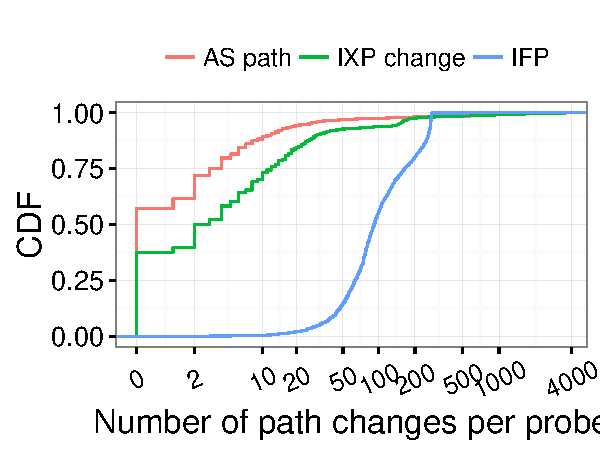
\includegraphics[width=\textwidth]{gfx/chap4/path_ch_count_cdf_cmp.pdf}
	\caption{\footnotesize CDF.}
	\label{fig:path_ch_count_cdf_cmp}
	\end{subfigure}
	\begin{subfigure}[b]{.48\textwidth}
	\centering
	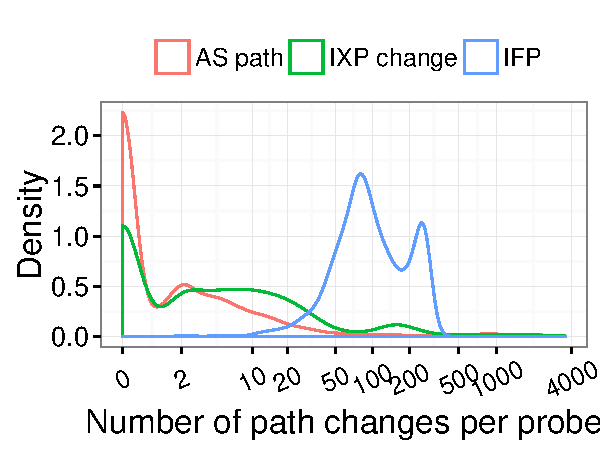
\includegraphics[width=\textwidth]{gfx/chap4/path_ch_count_density_cmp.pdf}
	\caption{\footnotesize Density.}
	\label{fig:path_ch_count_density_cmp}
	\end{subfigure}
\caption{Distribution of path change times per probe. One probe with most complete traceroute measurement is chosen for each AS. 2050 probes/ASes are included in the graph.}
\label{fig:path_ch_count_cmp}
\end{figure}

We consider only AS path changes where the difference starts from a hop position involving public ASNs in both AS paths.
Difference due to temporal presence of non-responding hops are ignored.
IXP change happens when the difference starts from a position involving at least one IXP hop in the two consecutive AS paths.
IRP changes are detected with \textit{backward extension}. 
Those overlap with any AS path/IXP changes are excluded, since they are potentially caused by intradomain routing changes.

The distribution of the number of path changes per probe trace is illustrated in Figure~\ref{fig:path_ch_count_cmp}.
One probe with the most complete traceroute measurements is selected for each of the 2050 source ASes.
1170 ($57.07\%$) of them experienced no AS path changes over the period of three months, indicating that the AS paths are in general very stable over time.
Still, 51 ($2.49\%$) probes underwent more than 100 AS path changes.
717 probes ($34.98\%$) didn't have any IXP change.
140 probes experienced frequent ($> 100$) IXP changes.
IRP changes are much more frequent than the other two path changes. 
Half of the selected probes experienced more than 90 IRP changes.
We investigate the nature of these path changes, together with their potential impact on RTT, in Section~\ref{sec:corr}.

\section{Match between RTT and path changes}
\label{sec:corr}

If a pair of RTT and path change on a same Internet path is close in time, chances are that the RTT change is caused by the path change. We say that these two changes are correlated or matched. 
%This is a demonstration of relevance between detected RTT change and underlying routing activities.
%We are interested in knowing the fraction/quantity of RTT and path changes that
However, there is no straightforward way matching the two types of change, as the measurement intervals are different: $30min$ for traceroute while $4min$ for ping. 

Again, \textit{minimum cost maximum-cardinality matching} appears to be a reasonable formulation of the correlation between RTT and path changes.
We therefore borrow the concept of optimal matching in changepoint evaluation (Section~\ref{sec:score}).
The shift tolerance window is set to the interval of traceroute measurement.
It is because causal relationship between the RTT and path change is possible (though not necessary) within that range.
A pair of RTT and path changes are correlated/matched if they are within in the so produced optimal matching.
The notion precision, introduced in section~\ref{sec:score}, is now interpreted as the fraction of path changes that are matched to an RTT change.
Recall now means the fraction of RTT changes that can be explained/matched to a certain type of path change.

We compare separately AS, IXP and \ac{IRP} path changes to RTT changes detected with \texttt{cpt\_np} and \texttt{cpt\_poisson}.
The matching is calculated for the 2050 probes mentioned in Figure~\ref{fig:path_ch_count_cmp}, each from a distinct AS.


\subsection{Forward or backward?}
\begin{figure}[!htb]
\centering
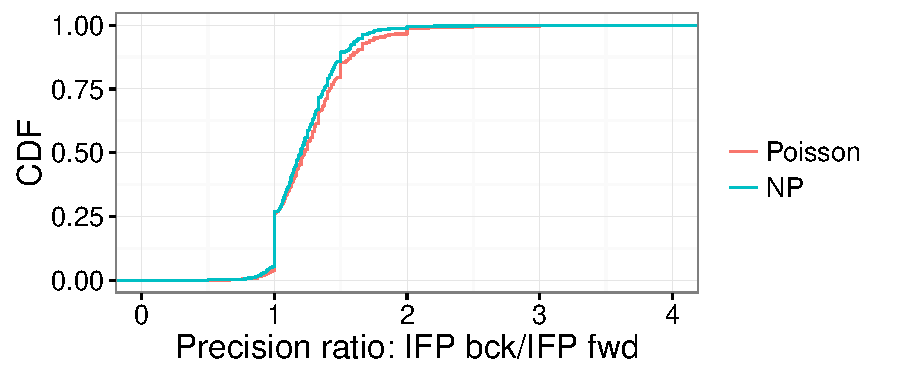
\includegraphics[width=.72\textwidth]{gfx/chap4/ifp_bck_ch_precision_gain_cdf.pdf}
\caption{Precision ration between IRP changes detected by \textit{backward extension} and \textit{forward inclusion}.}
\label{fig:IRP_bck_ch_precision_gain_cdf}
\end{figure}

In Section~\ref{sec:path}, two methods were presented to detect \ac{IRP} changes: \textit{backward extension} and \textit{forward inclusion}.
Do the \ac{IRP} changes detected with these two methods have any difference in terms of matching with RTT changes?
To answer this question, we compare for each probe the matching precision of these two methods.
The precision ratio between the two methods is given in Figure~\ref{fig:IRP_bck_ch_precision_gain_cdf}, in the form of CDF over probes.
\textit{backward extension} produces the same number of \ac{IRP} changes as \textit{forward inclusion} does.
However, \ac{IRP} changes by \textit{backward extension} are more likely to have a match with RTT changes for $75\%$ probes.
These probes are on the right side of the graph where the precision ration is bigger than 1.	
The significant increase in precision implies that the path changes detected by \textit{backward extension} are more accurate and are thus is a necessary improvement to the basic approach.
Later on, we refer always to changes detected by \textit{backward extension} when talking about \ac{IRP} changes.

\subsection{Summary of matching between path change and RTT change}

\begin{table}[!htb]
\caption{Number of RTT changes matched with a path change for the selected 2050 probes.}
\label{tab:corr_overview}
\centering
\footnotesize
\setlength{\tabcolsep}{0.5em}
\begin{tabular}{l|cc|c}
\toprule
& \texttt{cpt\_poisson} & \texttt{cpt\_np} & \# path changes\\
\midrule
AS path change & 11,794 & 6,380 & 51,282 \\
IXP change & 9,126 & 8,341 & 73,544\\
IRP change & 38,700 & 36,400 & 244,713\\
\midrule
\# RTT changes & 481,877 & 307,312 & \\
\bottomrule
\end{tabular}
\end{table}
Table~\ref{tab:corr_overview} details the number of matches between path and RTT changes.
Each cell tells the number of matches between the corresponding line (path change type) and column (RTT change detection method).
The last column contains the total number of path changes of each kind.
Similarly, the last line provides the total number of of RTT changes detected by the two methods.

The fraction of AS path changes matched to RTT changes by either detection method is much lower than the reported $72.5\%$ in \cite{Rimondini2014}.
It seems that AS path changes have less significant impact on RTT than previous understanding.
Is there something particular with our dataset or methods?
Moreover, the number of AS path changes match with \texttt{cpt\_np} RTT change is only about half of that with \texttt{cpt\_possion} RTT changes.
On the contrary, matching numbers for IXP and \ac{IRP} changes are quite close across the two RTT change detection methods.
Where does this difference come from?
All of these are very intriguing phenomena.
We try to explore the underlying reasons in the next section with a close-up look.

\section{Change detection sensitivity and relevance}
\subsection{\texttt{cpt\_poisson} matches better with AS path change?}
\label{sec:as_match_diff}
\begin{figure}[!htb]
\centering
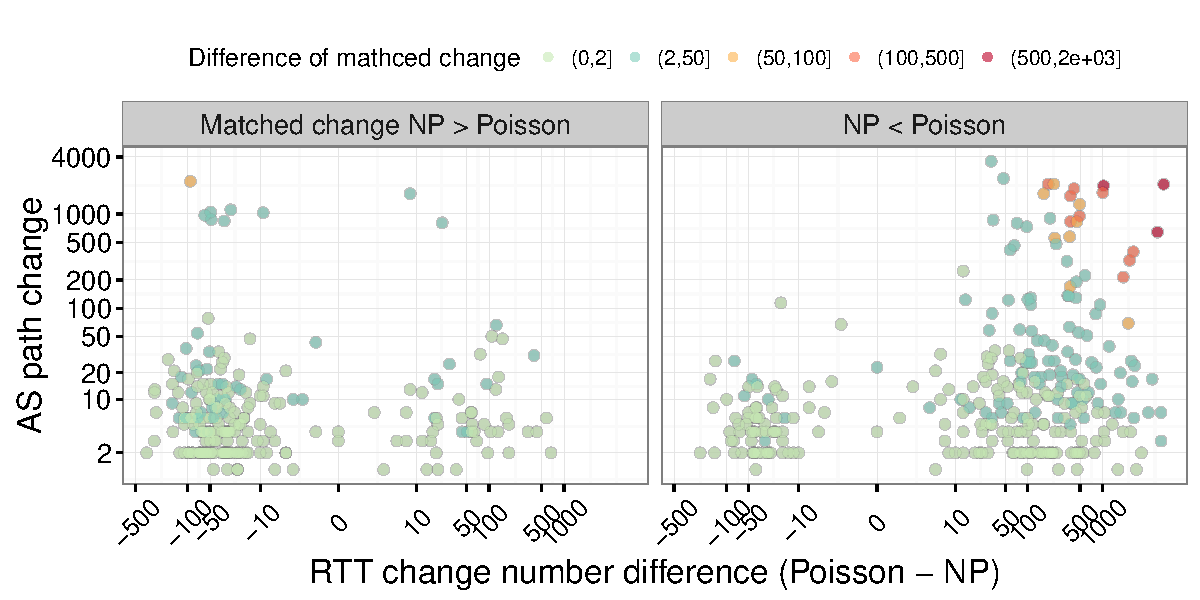
\includegraphics[width=.96\textwidth]{gfx/chap4/as_match_diff.pdf}
\caption{Probe having difference in the number of AS path changes matched to RTT changes detected by \texttt{cpt\_poisson} and \texttt{cpt\_np}. Probes are characterized by its AS path change numbers and RTT change number difference between the two methods. The color of each probe indicates the level of difference in matched change. Left panel shows the probes with more AS path changes matched to \texttt{cpt\_np} RTT changes.}
\label{fig:as_match_diff}
\end{figure}

It seems that there are much more \texttt{cpt\_poisson} RTT changes matched with AS path change, according to Table~\ref{tab:corr_overview}. But really?
Among the 880 probes ever experienced AS path changes, 293 probes have more AS path changes matched to \texttt{cpt\_poisson} RTT changes, 224 have more AS path changes matched to \texttt{cpt\_np} changes, 
Among the above mentioned 517 probes, 463 are actually with a difference smaller than 10 AS path changes.
The rest 363 (among the 880) probes have no difference across the two methods.

Contrary to what we see in Table~\ref{tab:corr_overview}, the numbers of AS path matched with RTT changes are in fact highly consistent across the two methods for the majority of probes.
The difference is caused by a small fraction of probes identified in Figure~\ref{fig:as_match_diff}.
In the graph, each dot represents one of the 880 probes that ever experienced AS path changes.
More reddish the dot (probe) is, larger the difference is between \texttt{cpt\_poisson} and \texttt{cpt\_np}.
We can tell from the graph that those probes plainly in red all experienced a large number of AS path changes (y-axis).
Moreover, when there is more \texttt{cp\_poisson} RTT changes (the positive side of the X-axis), it's more likely that more AS path changes from that probe are matched to \texttt{cp\_poisson} RTT changes as well(the left panel).
The reverse is as well true when there is more \texttt{cp\_np} RTT changes.
All together, the difference in matched RTT changes with AS path changes fundamentally lies in the difference of detection sensitivity (number of detected RTT changes) across different probe traces.
This difference is manifested through extremely frequent AS Path changes of several specific probes.


\subsection{Is \texttt{cpt\_poisson} more sensitive?}
\label{sec:over_sensitive}
\begin{figure}[!htb]
\centering
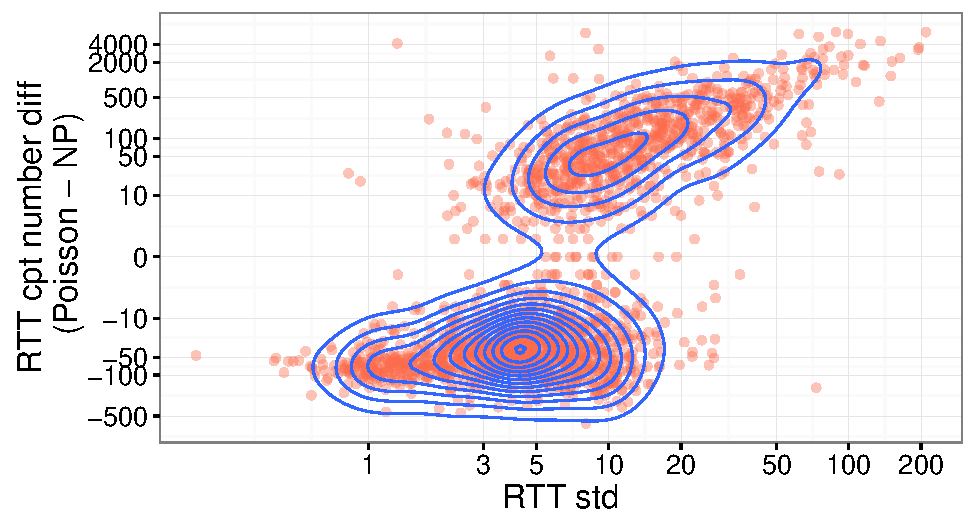
\includegraphics[width=.64\textwidth]{gfx/chap4/cpt_diff_vs_std.pdf}
\caption{Relation between RTT change number difference by the two changepoint method and the RTT trace $std$.}
\label{fig:cpt_diff_vs_std}
\end{figure}

\texttt{cpt\_poisson} detects in total more RTT changes than \texttt{cpt\_np}, according to Figure~\ref{fig:rtt_ch_count_density_cmp} and Table~\ref{tab:corr_overview}.
Therefore, \texttt{cpt\_poisson} seems to be more sensitive in change detection. But really?

With a per probe breakdown, we discovered that the number of RTT changes detected with the two methods is somehow related to the overall variation level of each probe trace.
This relationship is visualized in Figure~\ref{fig:cpt_diff_vs_std}.
Each dot represents a probe RTT timeseries. 
The X-axis indicates the RTT standard deviation in $msec$, while the Y-axis tells the difference in RTT changepoint numbers between the two methods.
Again, to facilitate the interpretation, we overlapped the graph with a 2-dimensional density estimation for the datapoints on the surface. Inner contours represent dense area.

For most probes traces with small overall RTT variation, \texttt{cpt\_np} is in fact more sensitive and detects more RTT changes, according to the figure.
This observation agrees with with Figure~\ref{fig:rtt_ch_count_density_cmp} in the sense that \texttt{cpt\_np} detects much more changes of small amplitude.

For probes with relatively large overall RTT variation, \texttt{cpt\_poisson} tends to be more sensitive and the difference in change number increases with the level of RTT variance.
With comprehensive manual inspection, we found that those RTT traces with high variance mostly underwent large amplitude RTT oscillations, many of which caused by ping timeouts. 
As human change detector, we also found very difficult to mark moments of change for these traces.

As a matter of fact, \texttt{cpt\_poisson} is not very flexible in adjusting detection sensitive according to the variation level of input timeseries.
For example, for a RTT timeseries that is full of large amplitude variations, 
we would expect a detection method to restrain a little bit.
This incapability is because the variation tolerance of a Poisson model is coupled with the the timeseries mean.
After removing the baseline, different RTT timeseries are actually of similar mean, thus leading to similar sensitivity.
For an overly noisy RTT timeseries, the `constant' sensitivity turns out to be a large number of changepoints.
Meanwhile, \texttt{cpt\_np} seems to be very elastic in detection sensitivity and less variant in the number of changepoints produced according to Figure~\ref{fig:rtt_ch_count_density_cmp}.

\subsection{How AS path changes match to RTT changes?}
\begin{figure}[!htb]
    \centering
    \begin{subfigure}[b]{.48\textwidth}
	\centering
	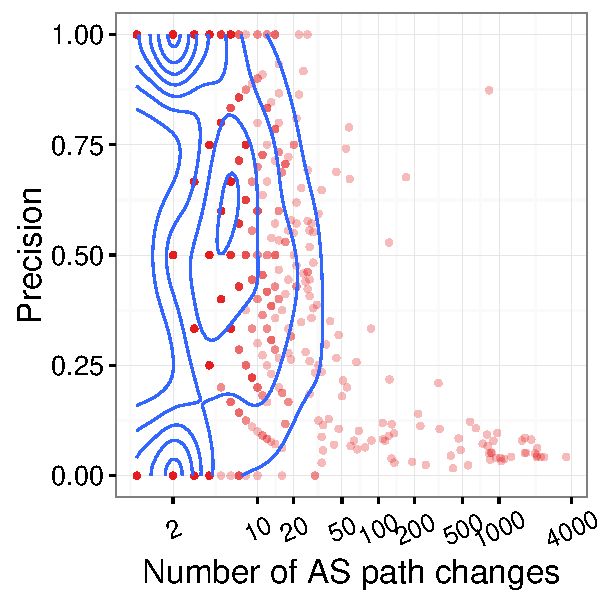
\includegraphics[width=\textwidth]{gfx/chap4/as_path_ch_precision_np.pdf}
	\caption{\footnotesize changes by \texttt{cpt\_np}.}
	\label{fig:as_path_ch_precision_np}
	\end{subfigure}
	\begin{subfigure}[b]{.48\textwidth}
	\centering
    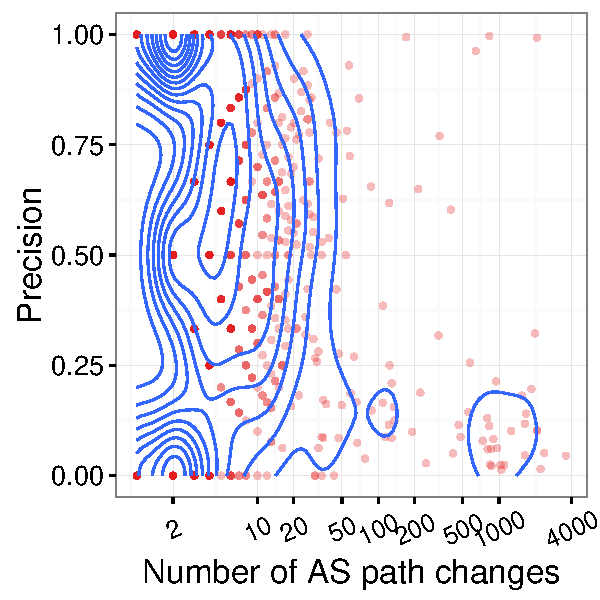
\includegraphics[width=\textwidth]{gfx/chap4/as_path_ch_precision_poisson.pdf}
	\caption{\footnotesize changes by \texttt{cpt\_poisson}.}
	\label{fig:as_path_ch_precision_poisson}
	\end{subfigure}
\caption{The relation between precision and AS path change times per probe trace.}
\label{fig:as_path_ch_precision}
\end{figure}

\begin{figure}[!htb]
\centering
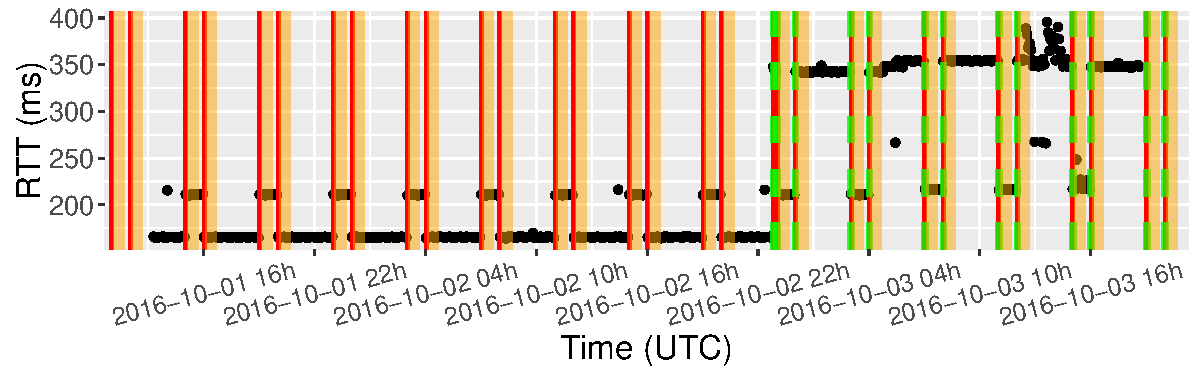
\includegraphics[width=.96\textwidth]{gfx/chap4/case_12849.pdf}
\caption{RTT from Probe 12849. Red lines for RTT change detected by \texttt{cpt\_poisson}; green dotted lines for RTT change by \texttt{cpt\_np}. Orange strips for AS path changes.}
\label{fig:case_12849_rtt}
\end{figure}

Two `bizarre' phenomena have been so far observed: 1) the match between AS path change and RTT change are much weaker than what reported in previous studies; 2) Certain ASes experienced extremely frequent AS paths changes.
Are these two somehow related?

We investigate this issue through a per probe breakdown between AS path change numbers and path change matching precision in Figure~\ref{fig:as_path_ch_precision}.
In the graph, each red dot represents a probe. The Y-axis tells the fraction of AS path changes that are matched to an RTT change, i.e. precision.
Since many probes (red dots) overlap with each other on the surface, we estimated the 2-dimensional distribution density and illustrated it with contour lines.
Inner contours are area with dense probes.

Figure~\ref{fig:as_path_ch_precision} reveals that probes with extremely frequent AS path changes (right side of the graphs) have in fact very low correlation, in terms of precision, with RTT changes.
After extensive manual inspection, those frequent AS path changes appear to be AS-level LB, i.e. the upstream AS employed in reaching the destination are switched very frequently among a few providers.
This could be a possible consequence of multipath BGP.
Such AS path changes generally don't have an obvious impact on RTT. 
For probes with fewer AS path changes (the left side of the graphs), the chance of having match between AS path change and RTT change is in fact pretty high.

Not all AS-level load balancing is without consequence. For example, probe 12849 in Figure~\ref{fig:case_12849_rtt} experienced 170 AS path changes, among which 169 are matched to RTT changes detected by \texttt{cpt\_poisson} and only 102 are matched to \texttt{cpt\_np} RTT changes.
These AS path changes are highly periodic and coincide with clear cut RTT changes.
\texttt{cpt\_np} failed to detect some of the changes with smaller amplitude.
The presence of such case confirms the need for measurement-based TE.
Otherwise, unwise routing decisions can be made without realization.

\subsection{Pitfalls of IXP and IRP path change detection}
Similar to AS path changes, probes with frequent IXP and IRP changes correlates weakly with RTT changes.
For example, in Figure~\ref{fig:path_ch_count_density_cmp}, there is a group of probes that experienced from 100 to 200 IXP changes. 
Only around $10\%$ of IXP changes on these probes are matched to an RTT change.

We investigate all the 58 probes in the area. These probe passed by AMS-IX to reach b-root most of the time. There were about 147 times, shared by these probes, where AMS-IX hop was replaced by a timeout hop before arriving at AS6939.
In such case, no IXP related address appears in the measured path. The presence of IXP is thus uncertain.
Still, we count it as an IXP change according to our definition in Section~\ref{sec:path}
\footnote{The newly released traIXroute v2.1 can detect IXP without the presence of IXP related IP address, if the neighbouring ASes are known to be member of a same IXP. However, it is still possible that two ASes peer at multiple IXPs, where the exact IXP traversed would remain uncertain.}.
This suggests that the detection of IXP changes are not very accurate, especially for those probes with many IXP changes.
This problem is stemmed from the difficulty of IXP inference in path measurements.


\begin{table}[!htb]
\caption{Quantiles of unique IP path numbers per probe trace.}
\label{tab:ip_path_count}
\centering
\footnotesize
\setlength{\tabcolsep}{0.5em}
\begin{tabular}{ccccccc}
\toprule
$5\%$ & $10\%$ & $25\%$ & $50\%$ & $75\%$ & $95\%$ & $100\%$\\
\midrule
20 & 32 & 56 & 91 & 145 & 419 & 4302\\
\bottomrule
\end{tabular}
\end{table}

The correlation of IRP changes with RTT changes are much weaker than that of AS and IXP path changes.
It turned out that most probes experienced much more than 16 end-to-end IP paths, according to Table.~\ref{tab:ip_path_count}.
In such case, one Paris ID might have been mapped to more than one IP paths.
This might lead to IRP changes without actual routing change.
Within in each single AS, the number of different IP paths rarely exceeds 16 toward a destination. 
However a chain of ASes can produce way much richer combinations of end-to-end IP paths.

Moreover, there is a group of probes having around 250 IRP changes according to Figure~\ref{fig:path_ch_count_density_cmp}.
An IRP change takes place roughly every 16 measurements on these probes. 
These changes are as well poorly correlated to RTT changes.
We investigated some probes in the area and found out the frequent changes aren't necessary related to the large amount of end-to-end paths.
For some probes, two neighbouring IRPs only differ at one or two Paris IDs.
IP paths taken by these Paris IDs oscillates between a few alternatives frequently.
For example, the Paris ID 6, 7, 8, 9 of probe 23998 switches a lot among only 2 paths.
Such change in general doesn't have obvious consequence on RTT level.

\subsection{Unmatched RTT changes}

\begin{figure}[!htb]
    \centering
    \begin{subfigure}[b]{.96\textwidth}
	\centering
	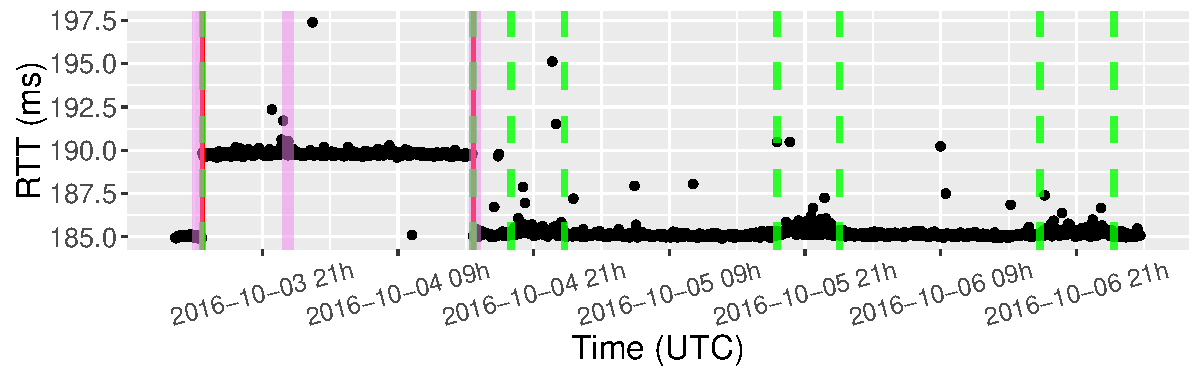
\includegraphics[width=\textwidth]{gfx/chap4/case_28002.pdf}
	\caption{\footnotesize Probe 28002.}
	\label{fig:case_28002}
	\end{subfigure}
	\begin{subfigure}[b]{.96\textwidth}
	\centering
	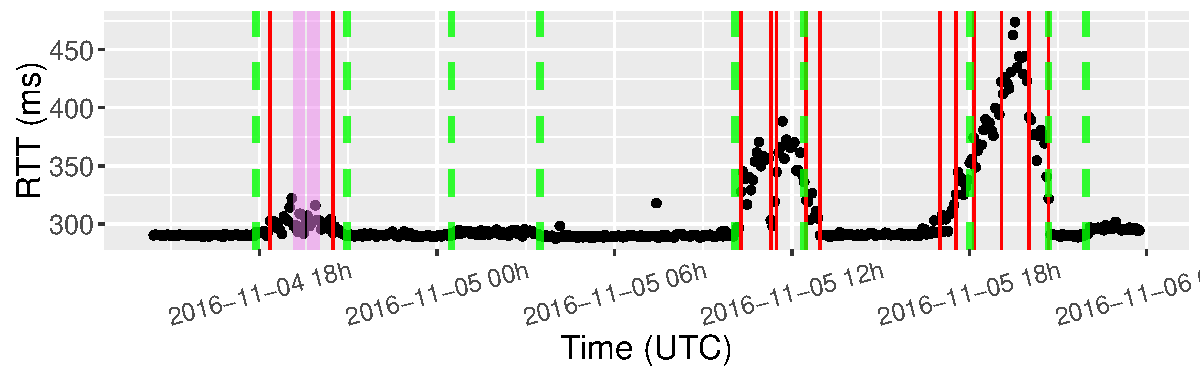
\includegraphics[width=\textwidth]{gfx/chap4/case_26328.pdf}
	\caption{\footnotesize Probe 26328.}
	\label{fig:case_26328}
	\end{subfigure}
\caption{RTT trace and change detection example. Red lines for RTT change detected by \texttt{cpt\_poisson}; green dotted lines for RTT change by \texttt{cpt\_np}. Violet strips are IRP changes.}
\label{fig:case_sensitivity}
\end{figure}

Several reasons contribute to the large amount and fraction of RTT changes unmatched to any path changes.
First, changes on the reverse path are not observed. 
We were not able to measure the reverse path with RIPE Atlas built-in measurement.
Therefore, it is impossible to detect the changes on the reverse path. 
However, these changes could have contributed to RTT changes. 
Especially in the context of inter-domain routing where paths are likely to be asymmetric.
This implies that the RTT changes caused by the reverse path changes are probably different from those caused by path changes on the forwarding direction.

Second, congestion. 
Congestion can be independent of path changes and yet is capable of causing significant RTT variations.
Figure~\ref{fig:case_26328} gives an typical example of RTT changes probably caused by congestion.
There are three bumps that can be visually noticed in the plotted RTT timeseries.
We say the latter two are probably congestion.
First, they do not correspond to any path changes, at least in the forwarding direction.
Second, these bumps are probably caused by filling queues along the path.
Because, the RTTs within these bumps are not flat.
On slightly loaded path, we would expect fairly constant RTT measurements overtime.
It is because the queues are almost empty, thus no room for delay variation.
On the other hand, the changing RTTs within the bump are probably a reflection of how the traffic demand on the bottleneck evolves due to end-to-end congestion control mechanism.
Both bumps/congestion deviate greatly from the baseline and last for a several hours.
They thus have significant impact on transmission performance.
We successfully detected them with the studied changepoint detection methods.
However, such detection is not possible with the previously proposed method~\cite{Luckie2014}.
It performs spectral analysis on RTT timeseries to find out periodically repeated congestion.
Such persistent congestion is normally due to lack of network capacity.
Meanwhile, transient congestion in Figure~\ref{fig:case_26328} is more likely caused by sudden traffic variations.
Measurement-based TE aims to avoid both types of congestion when there is alternative paths with available capacity.
For that purpose, changepoint detection methods are indeed helpful in notifying the presence of such performance variations. 

Third, over-sensitive detection.
If we boldly assume that path changes on reverse paths cause a comparable amount of RTT changes as forwarding path changes do, there are still many RTT change unmatched.
Some of them might be effectively attributed to congestion, as explained here above.
The remaining unmatched RTT changes are plainly the result of over-sensitive detection.
We already revealed from a macroscopic view, in Section~\ref{sec:cpt_trace} and ~\ref{sec:as_match_diff}, that \texttt{cpt\_poisson} tend to overestimate the number of changepoints when the RTT trace is noisy.
Meanwhile, \texttt{cpt\_np} is capable of detecting delicate RTT changes. 
Individual traces are given in Figure~\ref{fig:case_sensitivity} to illustrate the sensitivity difference from a microscopic view. 
In Figure~\ref{fig:case_28002}, \texttt{cpt\_np} detected all the periodic small amplitude congestion.
This is actually quite impressive, as these change are only hardly visible for human experts.
The changepoints marked by \texttt{cpt\_np} indeed highlighted their presence, and made them easier to be noticed visually.
In Figure~\ref{fig:case_26328}, both methods identified the two large bumps near the end of the timeseries.
The difference is that \texttt{cpt\_poisson} marked intermediate level changes as well.
These intermediate changepoints are clearly not correlated to any path changes.
On top of that, they are as well redundant in informing the congestion that was happening at that moment.
The reason for such over-sensitivity was due to its incompetence in adjusting the detection sensitivity according to input variance level. This issue is explored and explained in Section~\ref{sec:over_sensitive}.

\section*{Conclusion}
In this chapter, we proposed an evaluation framework for change detection on RTT time series.
The framework is robust with human-labeled dataset and weights RTT changes according to their importance in network operation. 
We further designed a data transformation adapted to RTT measurements to improve the detection sensitivity of some detection methods.
In detecting path changes, we distinguish those caused by routing changes from those due to load balancing.
Finally, we correlate the detected RTT and path changes by establishing an one-to-one matching between them. 
We investigated the sensitivity distinction across different change detection methods. 
Hidden issues with path changes are as well revealed.

This work is mere a facilitator for measurement-based TE. 
Further efforts are required in building a working system.
